\documentclass[11pt, a4paper]{article}

\usepackage{amsmath, amssymb, titling}
\usepackage[margin=2.5cm]{geometry}
\usepackage[colorlinks=true, linkcolor=black, urlcolor=black, citecolor=black]{hyperref}
\usepackage{graphicx}
\usepackage{caption}
\usepackage{subcaption}
\usepackage{float}
\usepackage{cancel}
\usepackage{fancyhdr, lastpage}
\usepackage{fourier-orns}
\usepackage{xcolor}
\usepackage{nomencl}
\makenomenclature
\usepackage{etoolbox}
\usepackage{sidecap}
\usepackage{adjustbox}

\sidecaptionvpos{figure}{c}
\setlength{\headheight}{18.2pt}
\setlength{\nomlabelwidth}{1.5cm}

% \renewcommand\maketitlehooka{\null\mbox{}\vfill}
% \renewcommand\maketitlehookd{\vfill\null}

\renewcommand{\headrule}{\vspace{-5pt}\hrulefill\raisebox{-2.1pt}{\quad\leafleft\decoone\leafright\quad}\hrulefill}
\newcommand{\parder}[2]{\frac{\partial {#1}}{\partial {#2}}}
% \renewcommand\nomgroup[1]{%
%   \item[\bfseries
%   \ifstrequal{#1}{F}{Far--Away Properties}{%
%   \ifstrequal{#1}{N}{Dimensionless Numbers}{%
%   \ifstrequal{#1}{M}{Matrices}{%
%   \ifstrequal{#1}{D}{Diagonals}{%
%   \ifstrequal{#1}{V}{Vectors}{%
%   \ifstrequal{#1}{P}{Dimensionless Average Properties}{}}}}}}
% ]}

\title{Numerical Methods in Aeronautical Engineering \\ HW1}
\author{Almog Dobrescu ID 214254252}

% \pagestyle{fancy}
\cfoot{Page \thepage\ of \pageref{LastPage}}

\begin{document}

\thispagestyle{empty}
\begin{figure}[H]
    \centering
    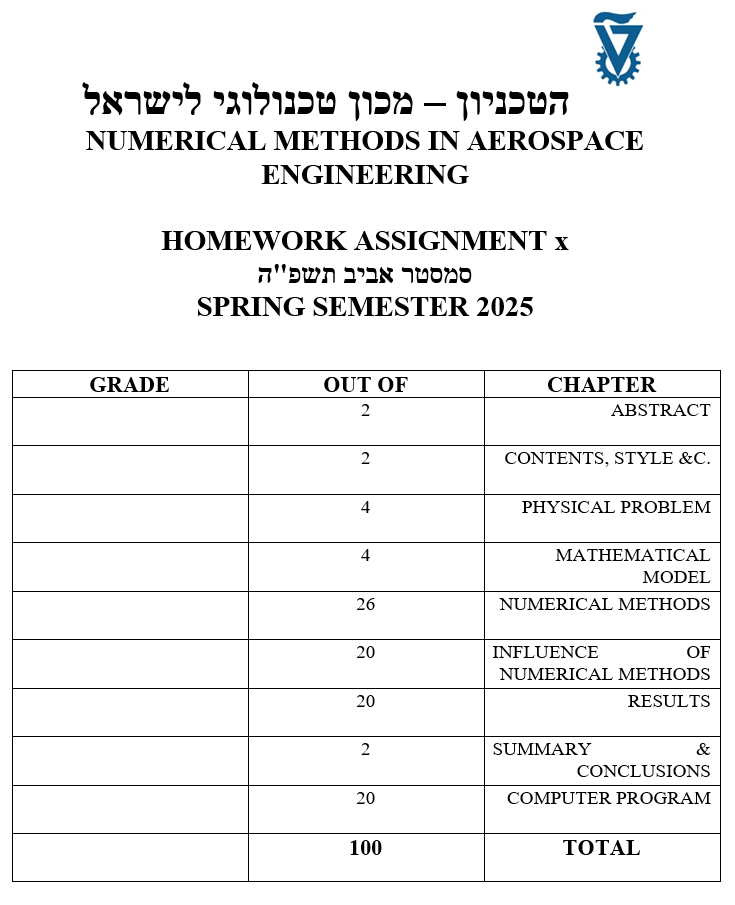
\includegraphics[width=\textwidth]{./../../../Cover page for computational assignments 2025.png}
    \label{fig: cover page}
\end{figure}
% \maketitle
\begin{center}
    \Huge
    Almog Dobrescu \qquad ID 214254252 \\ \vspace{0.5cm}
    \today
\end{center}
\newpage

\pagenumbering{roman}
% \setcounter{page}{1}
\begin{abstract}
    hello
\end{abstract}

\tableofcontents
\vfil
\listoffigures
\newpage

\printnomenclature
\newpage

\pagestyle{fancy}
\pagenumbering{arabic}
\setcounter{page}{1}

\section{The Physical Problem}
Liquid rockets are an important part of the future of rocket engine propulsion. To maximize the efficiency of the engine, it is crucial to know the location of the evaporation front. The physical problem at hand is the location of the evaporation front of a fuel spray after the atomization injector. 

\section{The Mathematical Model}
The evaporation front of fuel spray can be described by solving the following equations:
\begin{equation}
    \begin{array}{c}
        \displaystyle\frac{d^2T}{d\zeta^2}=\Lambda e^T\left(T_v-T_u+\alpha\beta-\frac{dT}{d\zeta}\right) \\\\
        \displaystyle m_d=\left(\alpha\beta\Lambda e^T\right)^{-1}\frac{d^2T}{d\zeta^2}
    \end{array}
    \label{eq: mathematical model}
\nomenclature{$x$}{spatial coordinate}
\nomenclature{$T$}{temperature}
\nomenclature{$m_d$}{mass fraction of liquid fuel in droplets}
\nomenclature{$T_v$}{vaporization temperature of the liquid fuel}
\nomenclature{$T_u$}{environment temperature of the liquid fuel upstream}
\nomenclature{$\Lambda$}{empirical constant of droplet vaporation}
\nomenclature{$\alpha$}{mass ratio between the liquid fuel and environment oxigen}
\nomenclature{$\beta$}{ratio between the latent heat of the liquid fuel and between the chemical reaction heat of liquid vapor with oxigen}
\end{equation}
The boundary condition of the problem:
\begin{equation}
    \begin{array}{lccl}
        \begin{matrix}
            \zeta\rightarrow-\infty: && m_d\rightarrow1 \\
            \zeta\rightarrow+\infty: && T\rightarrow\zeta\cdot\left(T_v-T_u+\alpha\beta\right)
        \end{matrix} &&& \begin{matrix}
            T & \rightarrow & \zeta\cdot\left(T_v-T_u\right) \\
            m_d & \rightarrow & 0
        \end{matrix}
    \end{array}
\end{equation}
\begin{itemize}
    \item According to the defenition of $T$: $\left.T\right|_{\zeta=0}=0$
\end{itemize}

\section{The Numerical Methods}
Eq.\ref{eq: mathematical model} can be rewrite as:
\begin{equation*}
    \displaystyle\frac{d^2T}{d\zeta^2}+\Lambda e^T\frac{dT}{d\zeta}-\Lambda e^T\left(T_v-T_u+\alpha\beta\right)=0
    \label{eq: the ode}
\end{equation*}
In our case:
\begin{itemize}
    \item $\infty$ is at around $30$
    \item $\Lambda=0.1$
    \item $T_v=0.203$
    \item $T_u=0.152$
    \item $\alpha\beta=0.0234$
\end{itemize}
To make sure that $\left.T\right|_{\zeta=0}=0$, we will solve the ODE in two steps, one from $\zeta\rightarrow-\infty$ to $\zeta=0$ and the second from $\zeta=0$ to $\zeta\rightarrow\infty$.

\subsection{Finite Difference Method}
Using central difference we can write the difference equations:
\begin{equation}
    \begin{array}{c}
        \displaystyle\frac{T_{i+1}-2T_i+T_{i-1}}{h^2}+\Lambda e^{T_i}\frac{T_{i+1}-T_{i-1}}{2h}-\Lambda e^{T_i}\left(T_v-T_u+\alpha\beta\right)=0 \hspace{1cm} \emph{O}\left(h^2\right) \\\\
        \begin{matrix}
            i=1,2,\cdots,N &&& \displaystyle h=\frac{\left.\zeta\right|_{i=N+1}-\left.\zeta\right|_{i=0}}{N+1-0}
        \end{matrix} 
    \end{array}
    \nomenclature{$h$}{size of each cell in the domain}
    \nomenclature{$i$}{cell index}
    \nomenclature{$N$}{number of elements}
\end{equation}
We will use the 'explicit point Jacobi' method:
\begin{enumerate}
    \item Set the filed with initial condition (linear interpolation).
    \item Calculate the temperature at index \emph{i} and time step \emph{n+1} from the previous time step:
    \begin{equation}
        \begin{array}{c}
            \displaystyle T_i^{n+1}=\frac{1}{2}\left(T_{i+1}^n+T_{i-1}^n\right)+\frac{h}{4}\Lambda e^{T_i^n}\left(T_{i+1}^n-T_{i-1}^n\right)-\frac{h^2}{2}\Lambda e^{T_i^n}\left(T_v-T_u+\alpha\beta\right)
        \end{array}
    \end{equation}
    \item The solution is considered converged when:
    \begin{equation}
        \left|T_i^{n+1}-T_i^n\right|<\varepsilon \hspace{1cm} \forall i\in[1, N]
        \nomenclature{$\varepsilon$}{convergence limit}
    \end{equation}
\end{enumerate}

\subsection{Shooting Method}
Let's rewrite Eq.\ref{eq: the ode} as a system of 2 ODE:
\begin{equation}
    \begin{matrix}
        \left\{\begin{array}{lcl}
            \displaystyle\frac{dT}{d\zeta} & = & s \\\\
            \displaystyle\frac{ds}{d\zeta} & = & -\Lambda e^Ts-\Lambda e^{T}\left(T_v-T_u+\alpha\beta\right)
        \end{array}\right. && \begin{array}{l}
            \left.T\right|_{\zeta\rightarrow-\infty}\rightarrow\zeta\cdot\left(T_v-T_u\right) \\\\
            \left.T\right|_{\zeta\rightarrow+\infty}\rightarrow\zeta\cdot\left(T_v-T_u+\alpha\beta\right)
        \end{array}
    \end{matrix}
    \nomenclature{$s$}{temporery variable}
\end{equation}
To solve the system of equations using the shooting method, we will guess $s_{(i=0)}^{(n)}$ and solve the system of equations using forward and backward differences (semi-implicit Euler). Namely:
\nomenclature{\fbox{$\cdot$}$^{(n)}$}{value at time step n}
\begin{equation}
    \begin{matrix}
        \left\{\begin{array}{lclr}
            \displaystyle s_{i+1}^{(n)} & = & \left(-\Lambda e^{T_i^{(n)}}s_i^{(n)}+\Lambda e^{T_i^{(n)}}\left(T_v-T_u+\alpha\beta\right)\right)\cdot h+s_i^{(n)} & \emph{O}\left(h\right)\\\\
            \displaystyle T_{i+1}^{(n)} & = & s_i^{(n+1)}\cdot h+T_i^{(n)} & \emph{O}\left(h\right)
        \end{array}\right. & \begin{array}{l}
            s_{i=0}^n=s_0^n \\\\
            T_{i=0}^n=\zeta\cdot\left(T_v-T_u+\alpha\beta\right) \\\\
            i=0,1,\cdots,N
        \end{array}
    \end{matrix}
\end{equation}
To correct the guess of $s_{(i=0)}^{(n)}$, let's define:
\begin{equation}
    F_{\left(s_{(i=0)}\right)}=T^{(n)}_{(i=N+1)}-\left.T\right|_{\zeta\rightarrow+\infty}
\end{equation}
\begin{itemize}
    \item When $F=0$, the guess of $s_{(i=0)}^{(n)}$ is correct
\end{itemize}
The next guess of \emph{s} $s_{(i=0)}^{(n+1)}$ will be calculated numerically by using a method to find the root of an equation. Namely:
\begin{equation}
    s_{(i=0)}^{(n+1)}=s_{(i=0)}^{(n)}-F_{\left(s_{(i=0)}^{(n)}\right)}\cdot\frac{s_{(i=0)}^{(n)}-s_{(i=0)}^{(n-1)}}{F_{\left(s_{(i=0)}^{(n)}\right)}-F_{\left(s_{(i=0)}^{(n-1)}\right)}} \hspace{1cm}\emph{O}\left(h\right)
\end{equation}

\section{Influence of The Numerical Methods}
\label{sec: Influence of The Numerical Methods}
\subsection{Finite Difference Method}
\subsubsection{Influence of number of elements N}
\begin{figure}[H]
    \centering
    \begin{subfigure}[c]{0.49\textwidth}
        \centering
        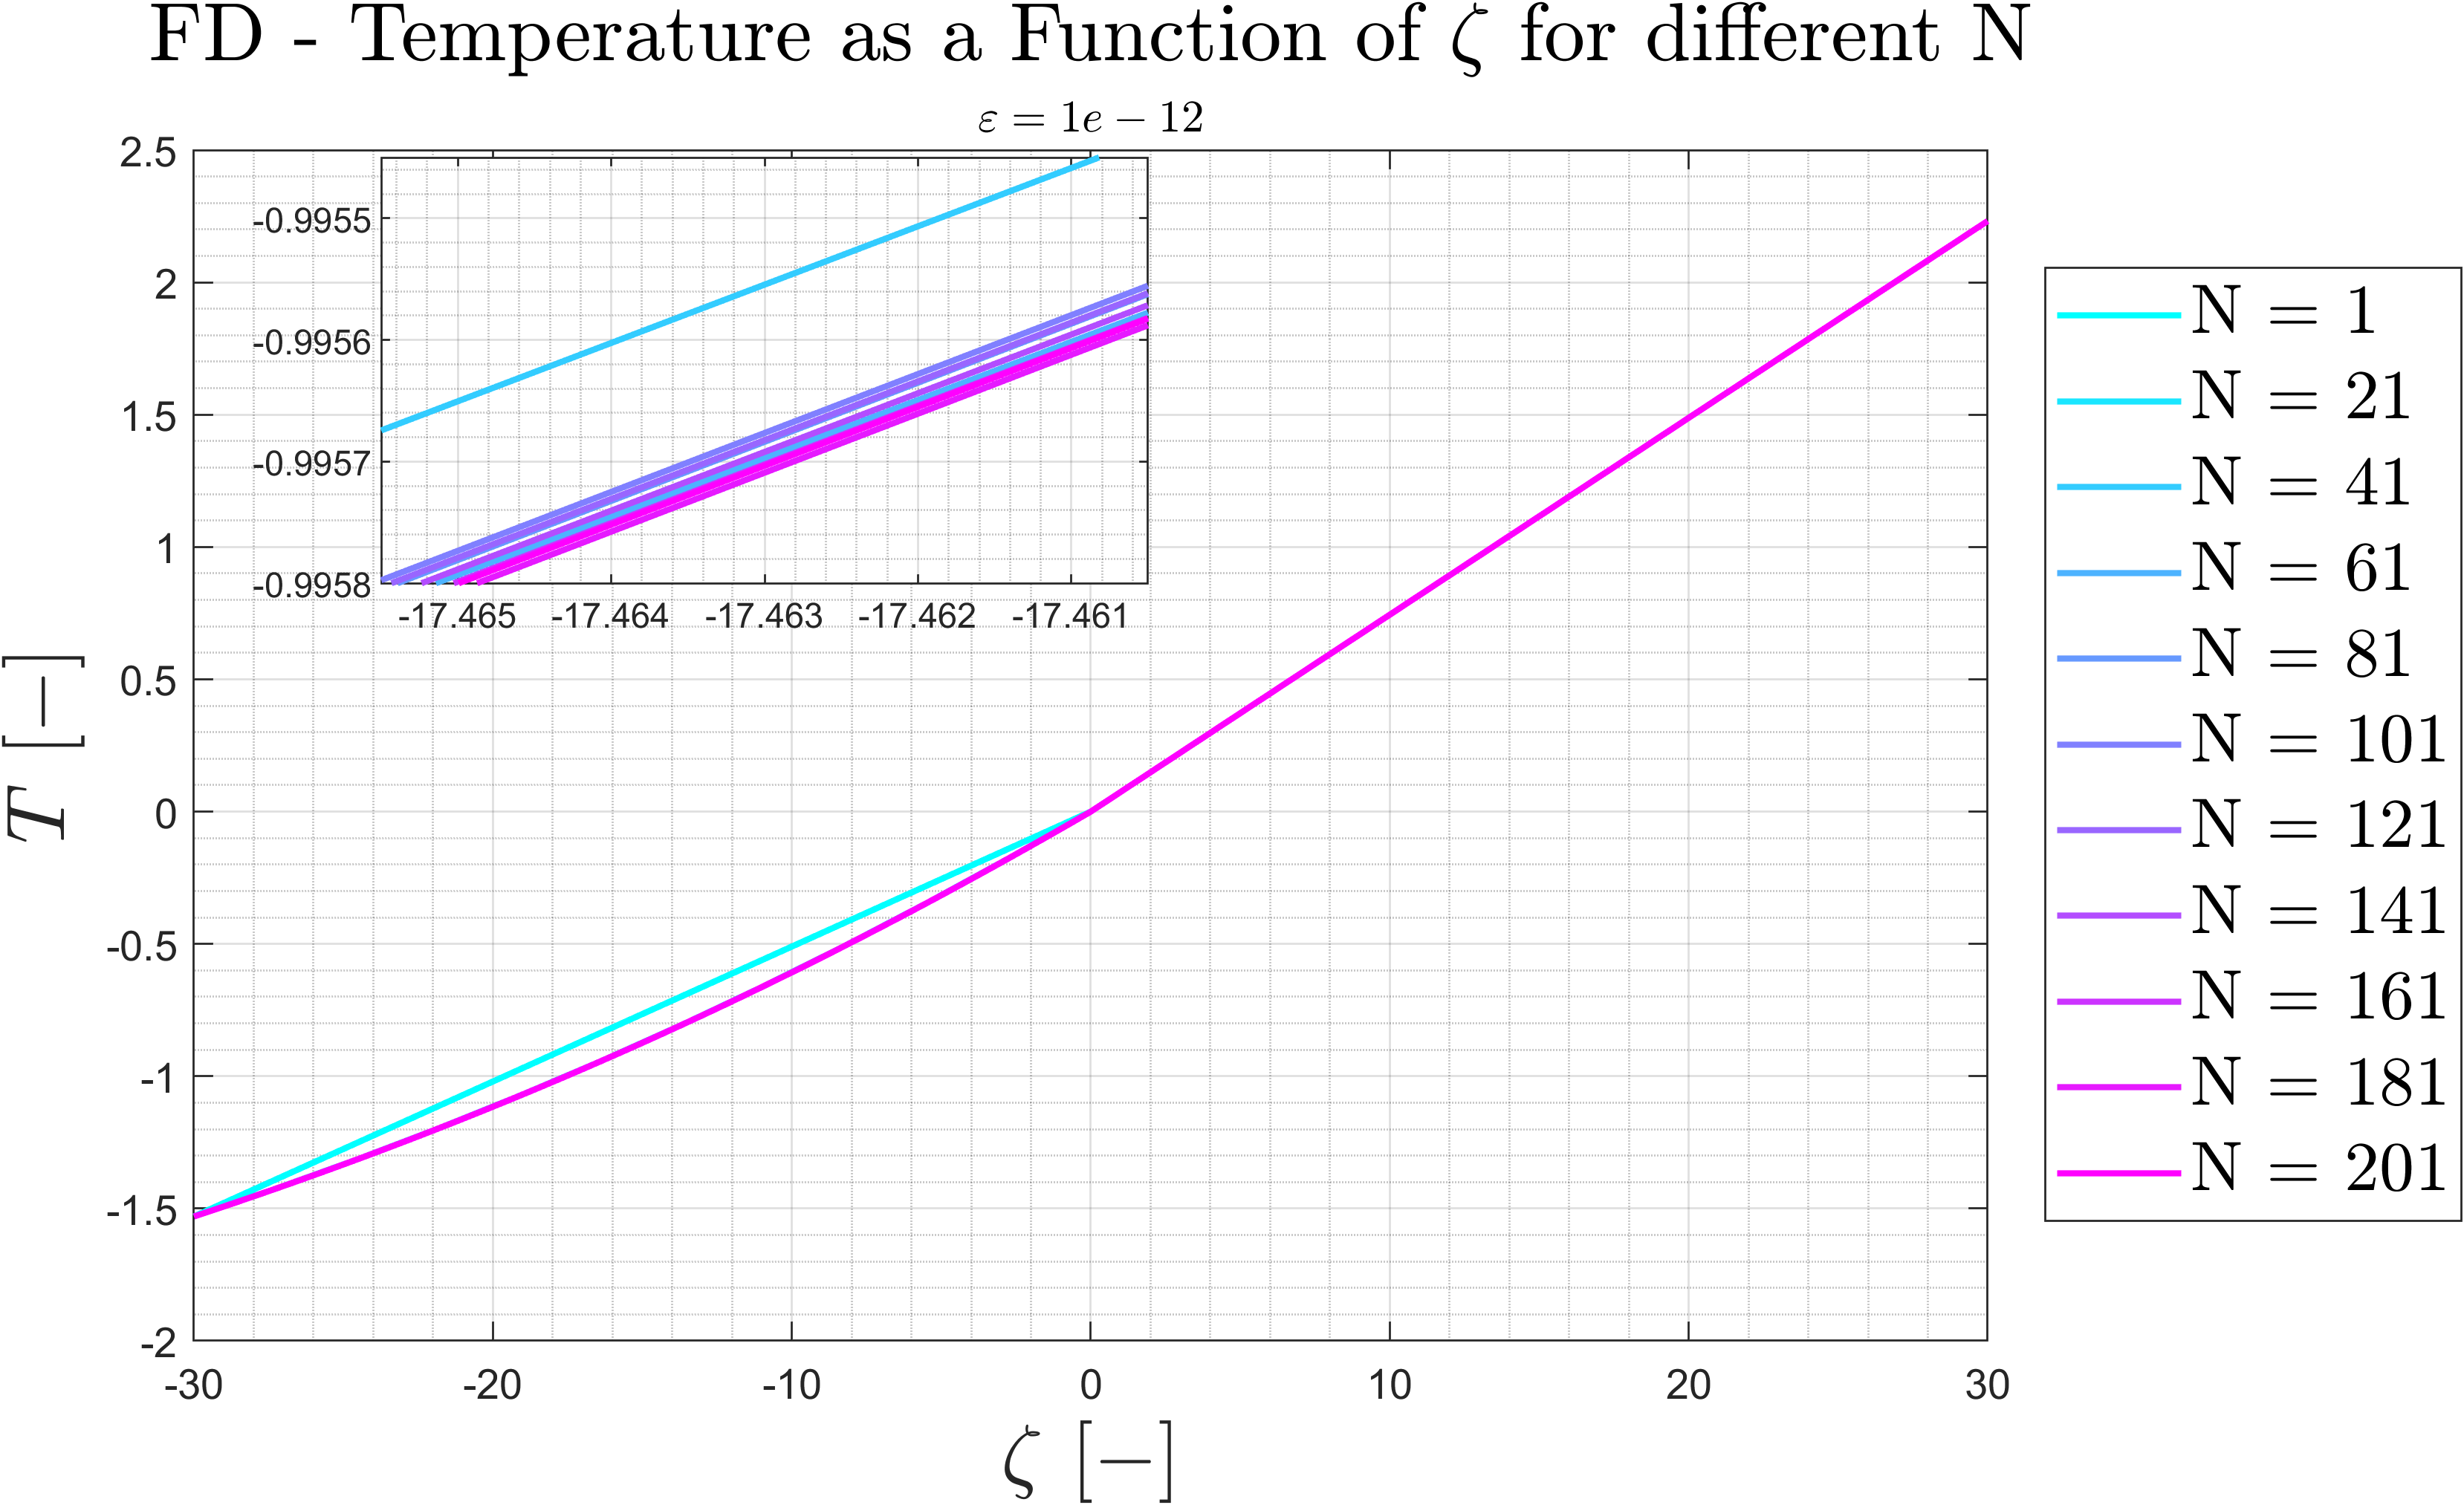
\includegraphics[width=\textwidth]{images/FD - T vs zeta for diff N.png}
        \caption{Temperature as a Function of $\zeta$ for different N}
        \label{fig: FD - T vs zeta for diff N}
    \end{subfigure}
    \hfill
    \begin{subfigure}[c]{0.49\textwidth}
        \centering
        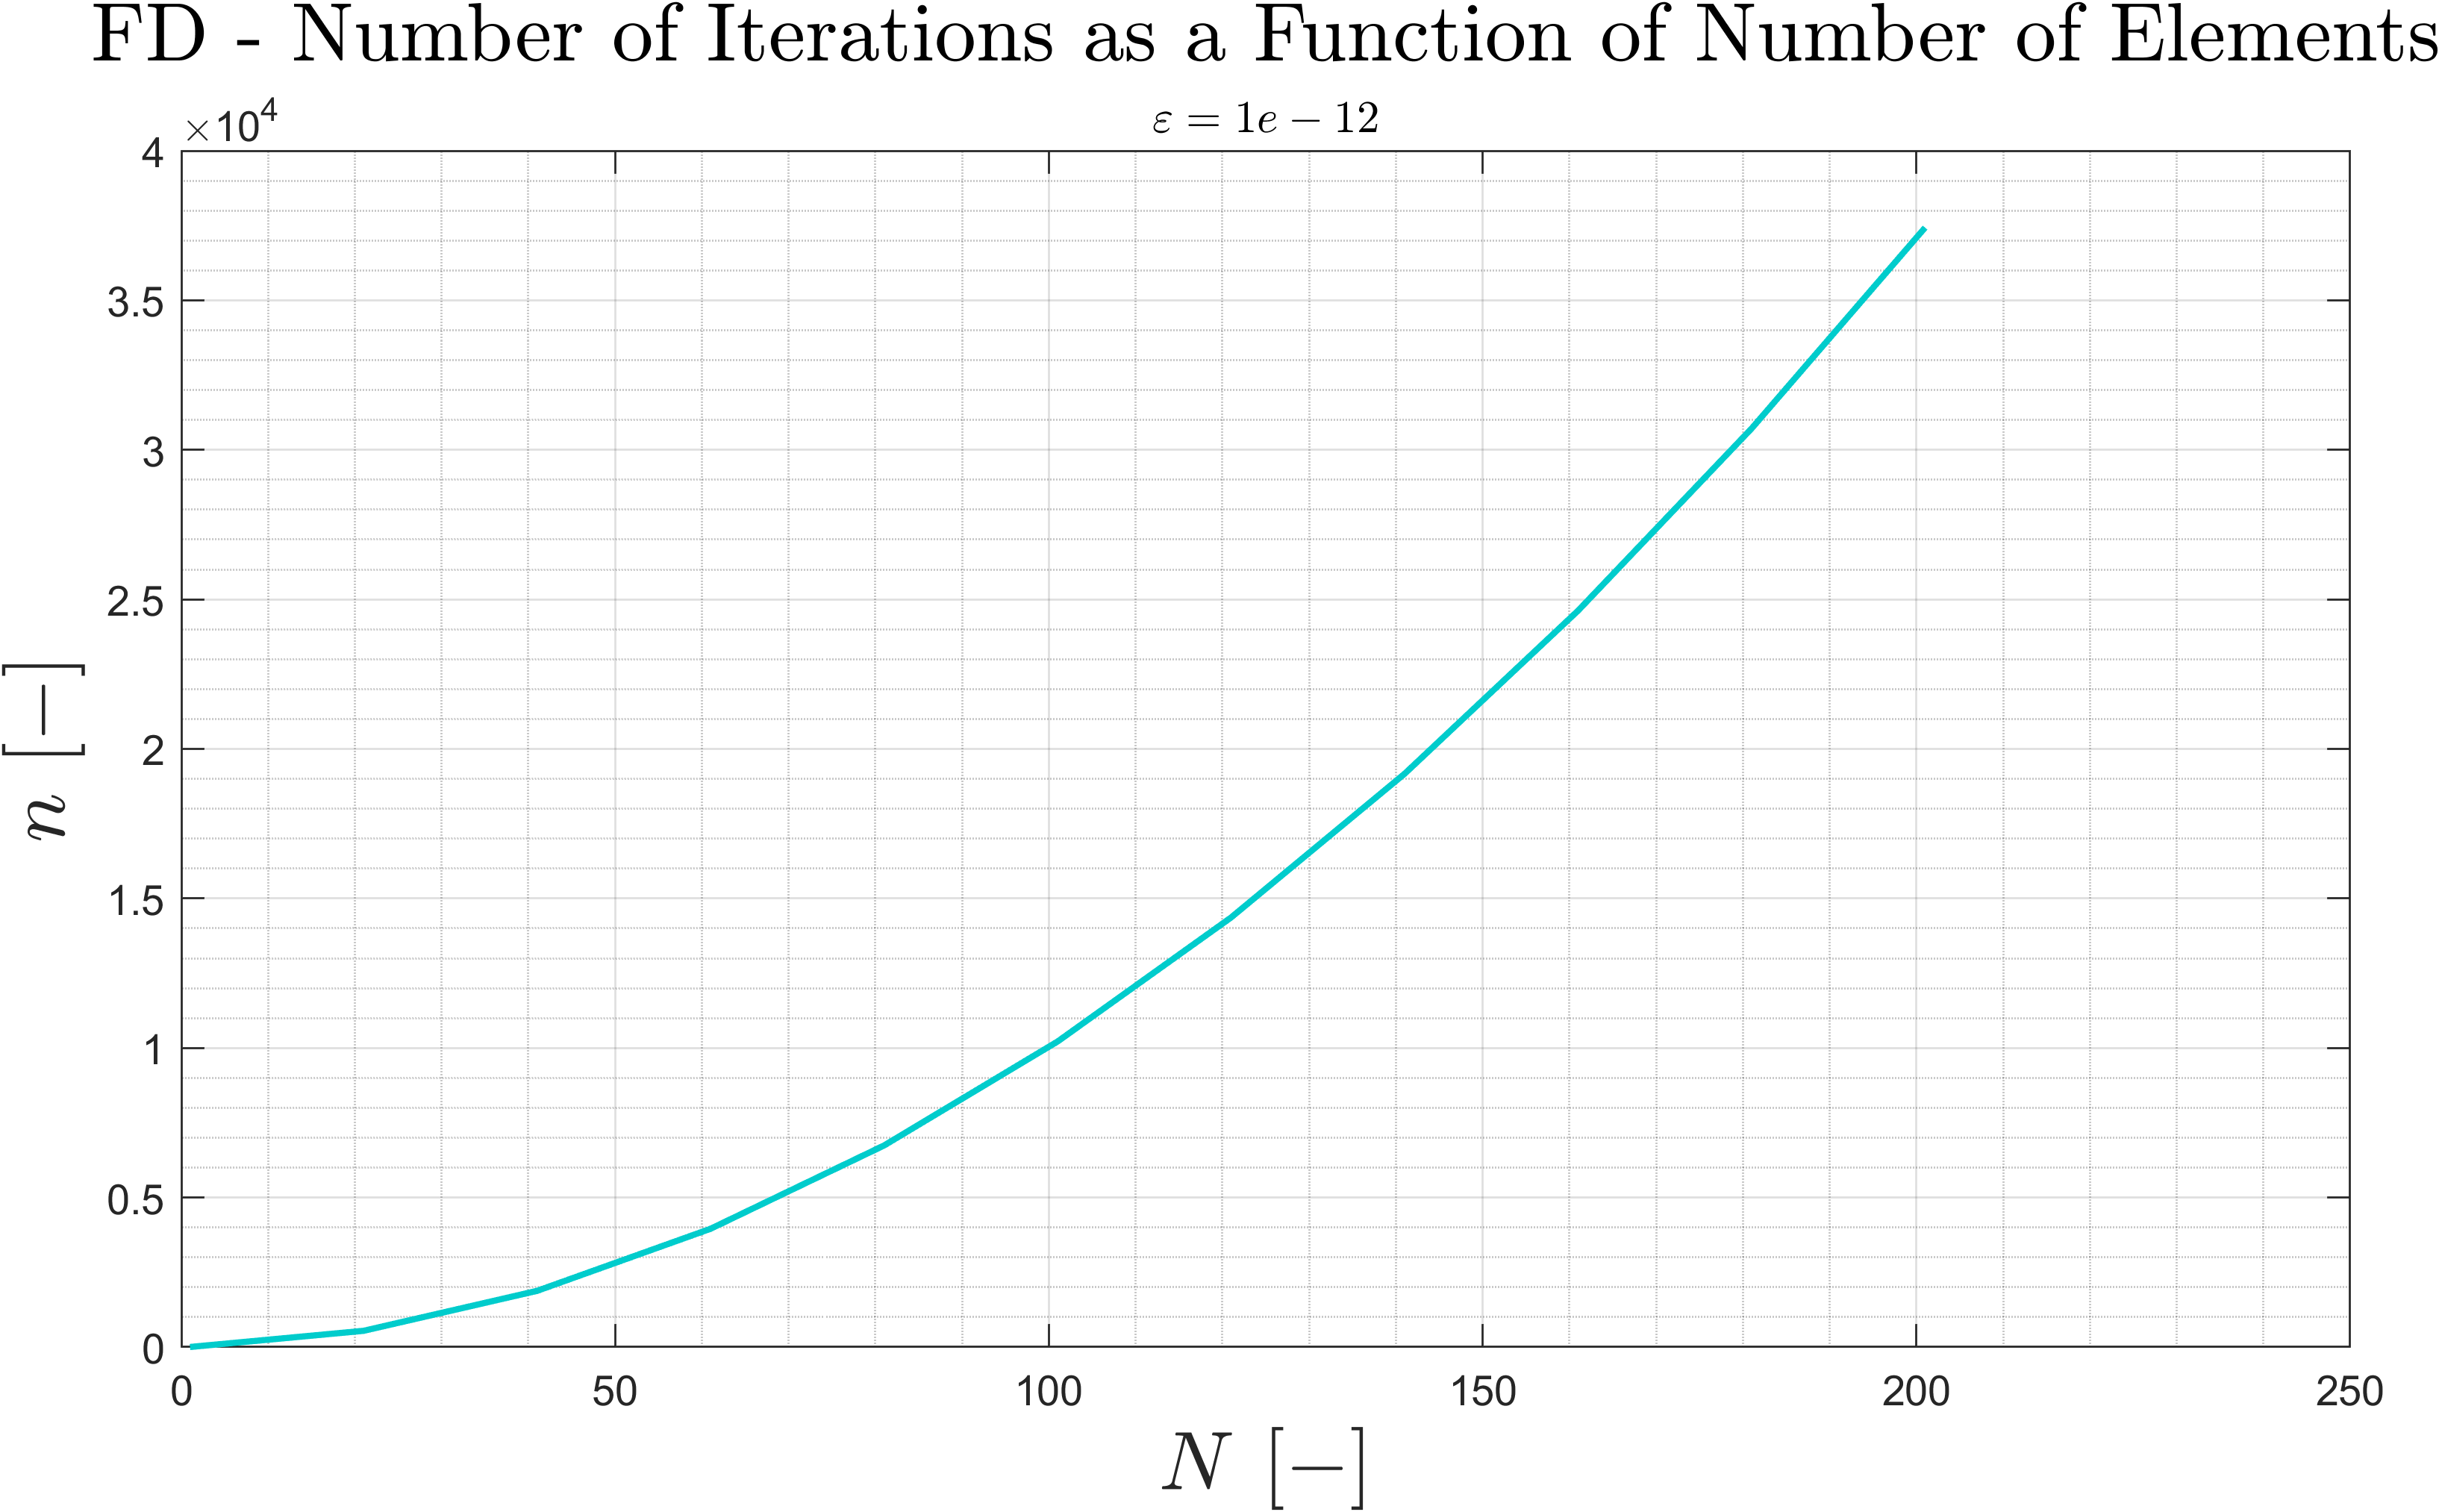
\includegraphics[width=\textwidth]{images/FD - n vs N.png}
        \caption{Number of iterations as a function of N}
        \label{fig: FD - n vs N}
    \end{subfigure}
    \caption{FD - Influence of the number of elements N}
    \label{fig: FD - Influence of N}
\end{figure}
In Fig.\ref{fig: FD - T vs zeta for diff N} we can see that for N bigger than 100, the solution does not really change. From Fig.\ref{fig: FD - n vs N} we can see that as the number of elements increases, the number of iterations increases as well. We can conclude that $N=101$ is a sufficient number of elements.

\subsubsection{Influence of convergence criteria $\varepsilon$}
\begin{figure}[H]
    \centering
    \begin{subfigure}[c]{0.49\textwidth}
        \centering
        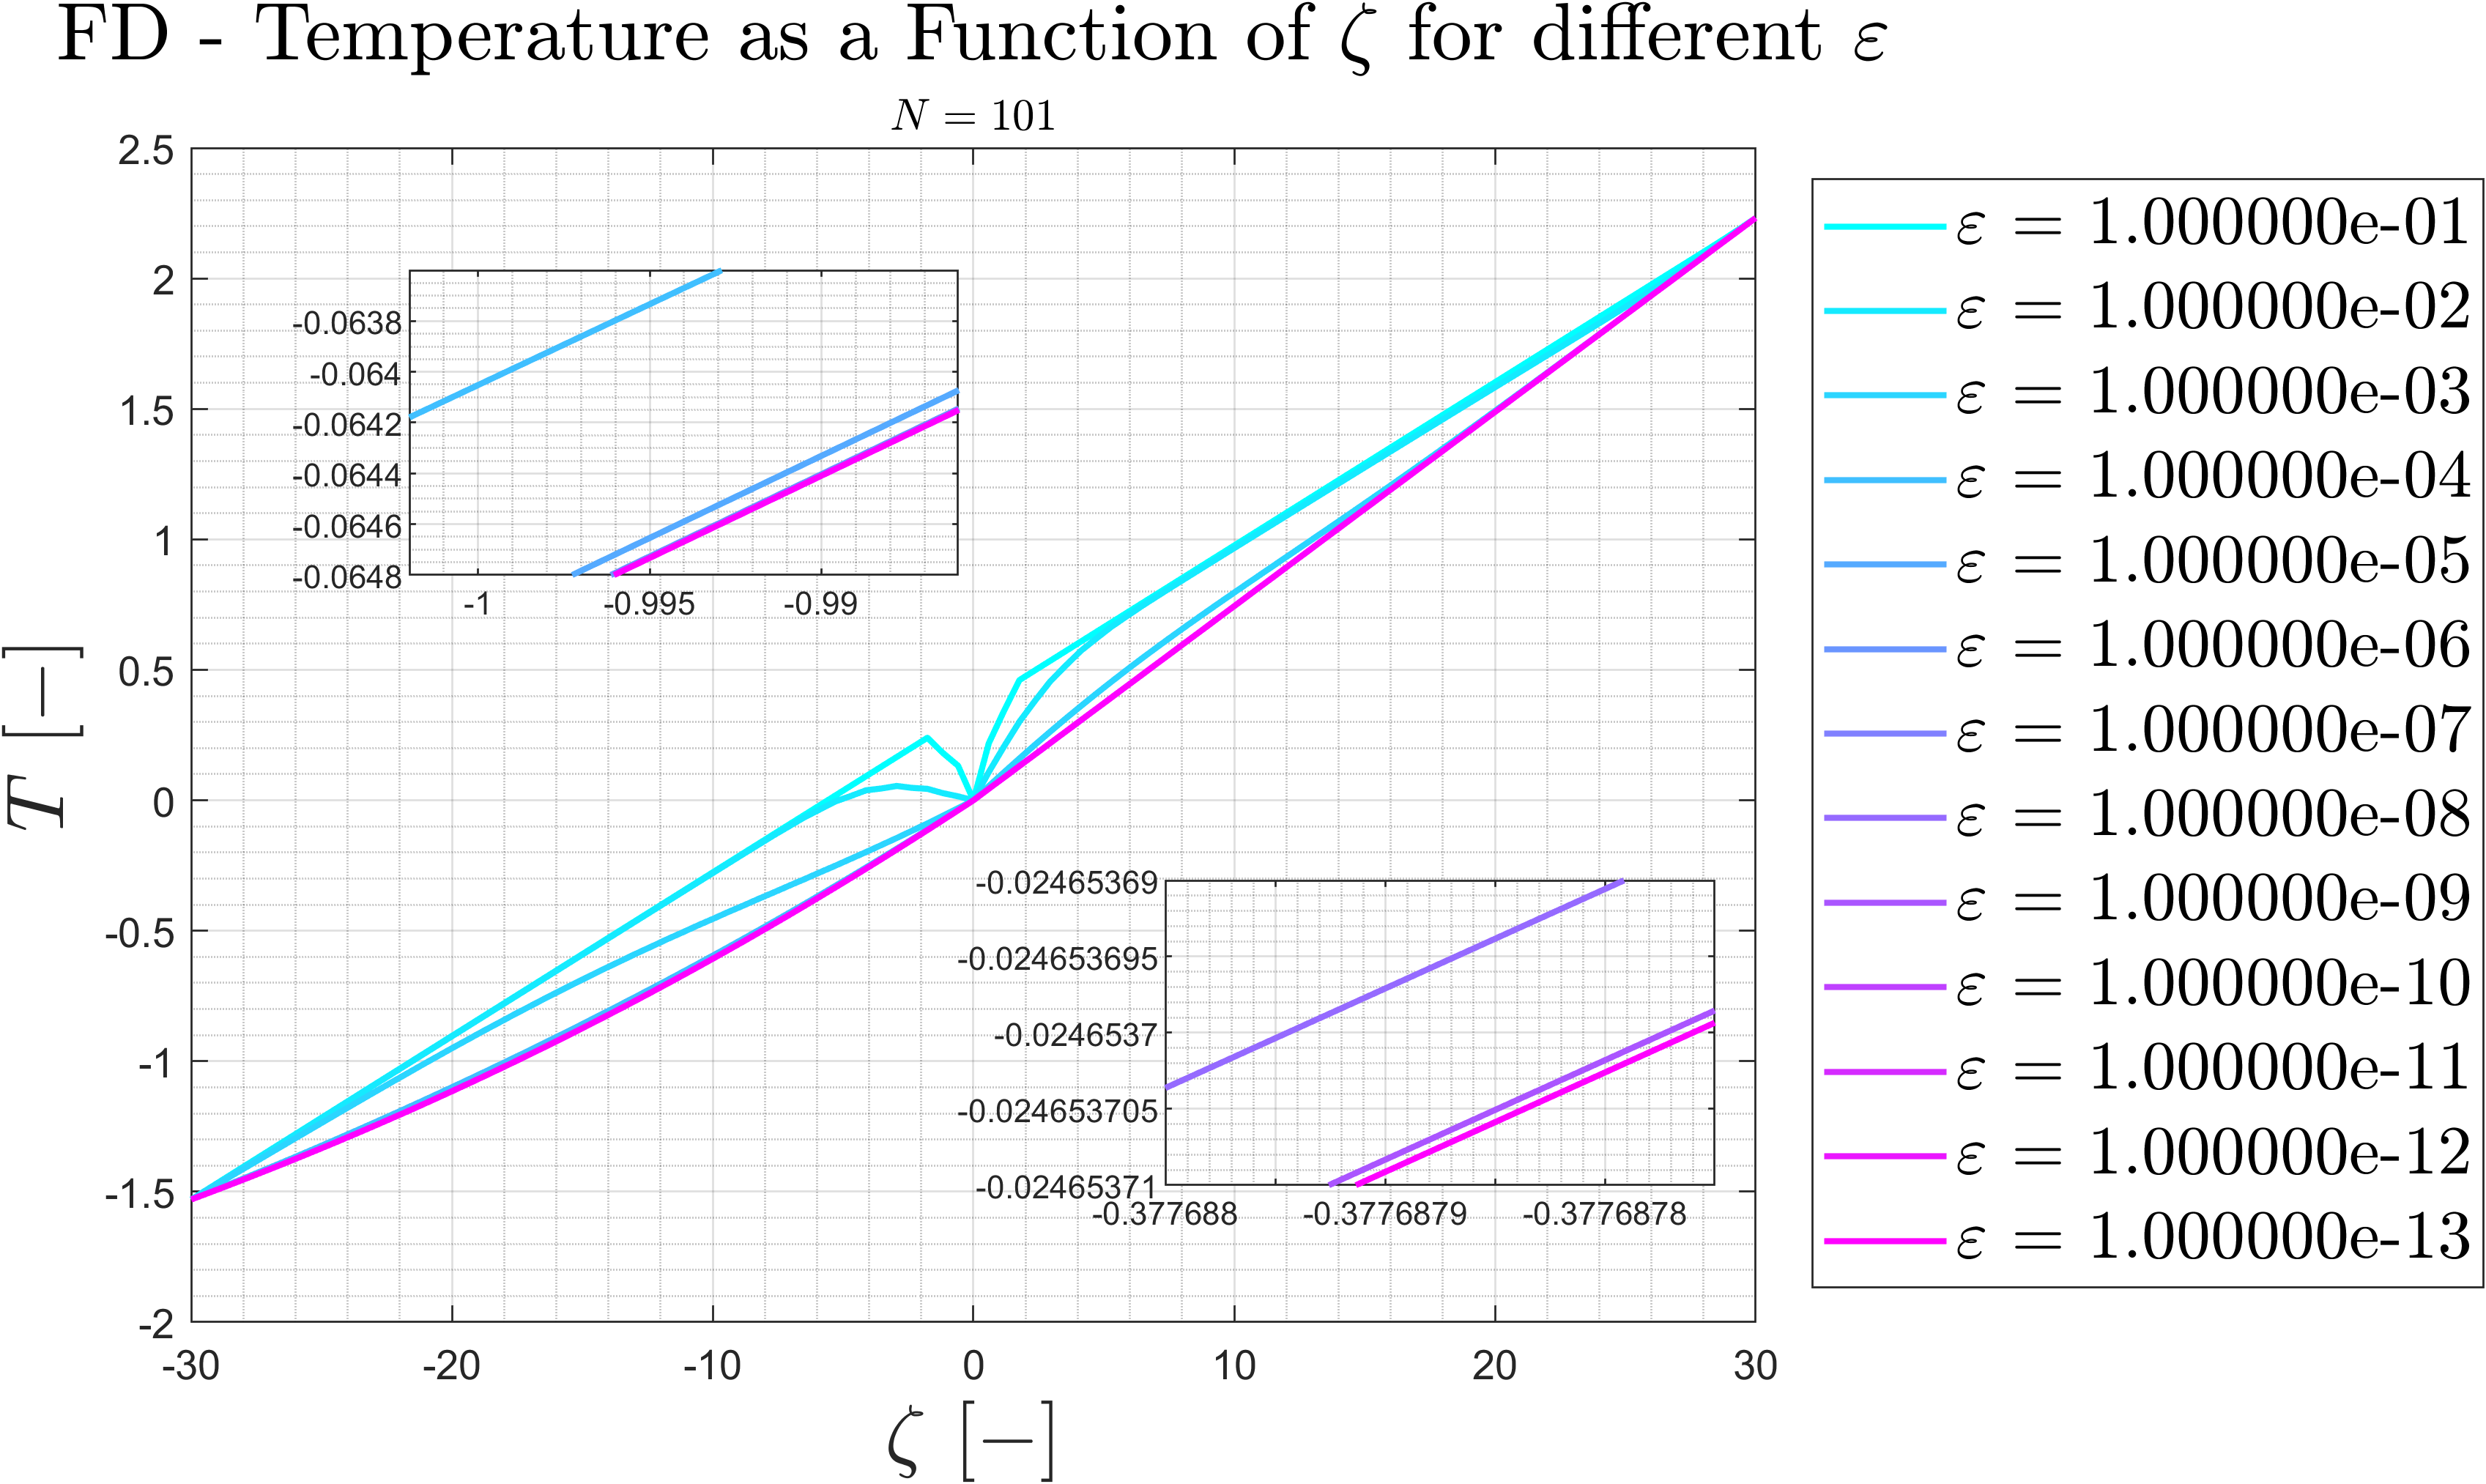
\includegraphics[width=\textwidth]{images/FD - T vs zeta for diff epsilon.png}
        \caption{Temperature as a Function of $\zeta$ for different $\varepsilon$}
        \label{fig: FD - T vs zeta for diff epsilon}
    \end{subfigure}
    \hfill
    \begin{subfigure}[c]{0.49\textwidth}
        \centering
        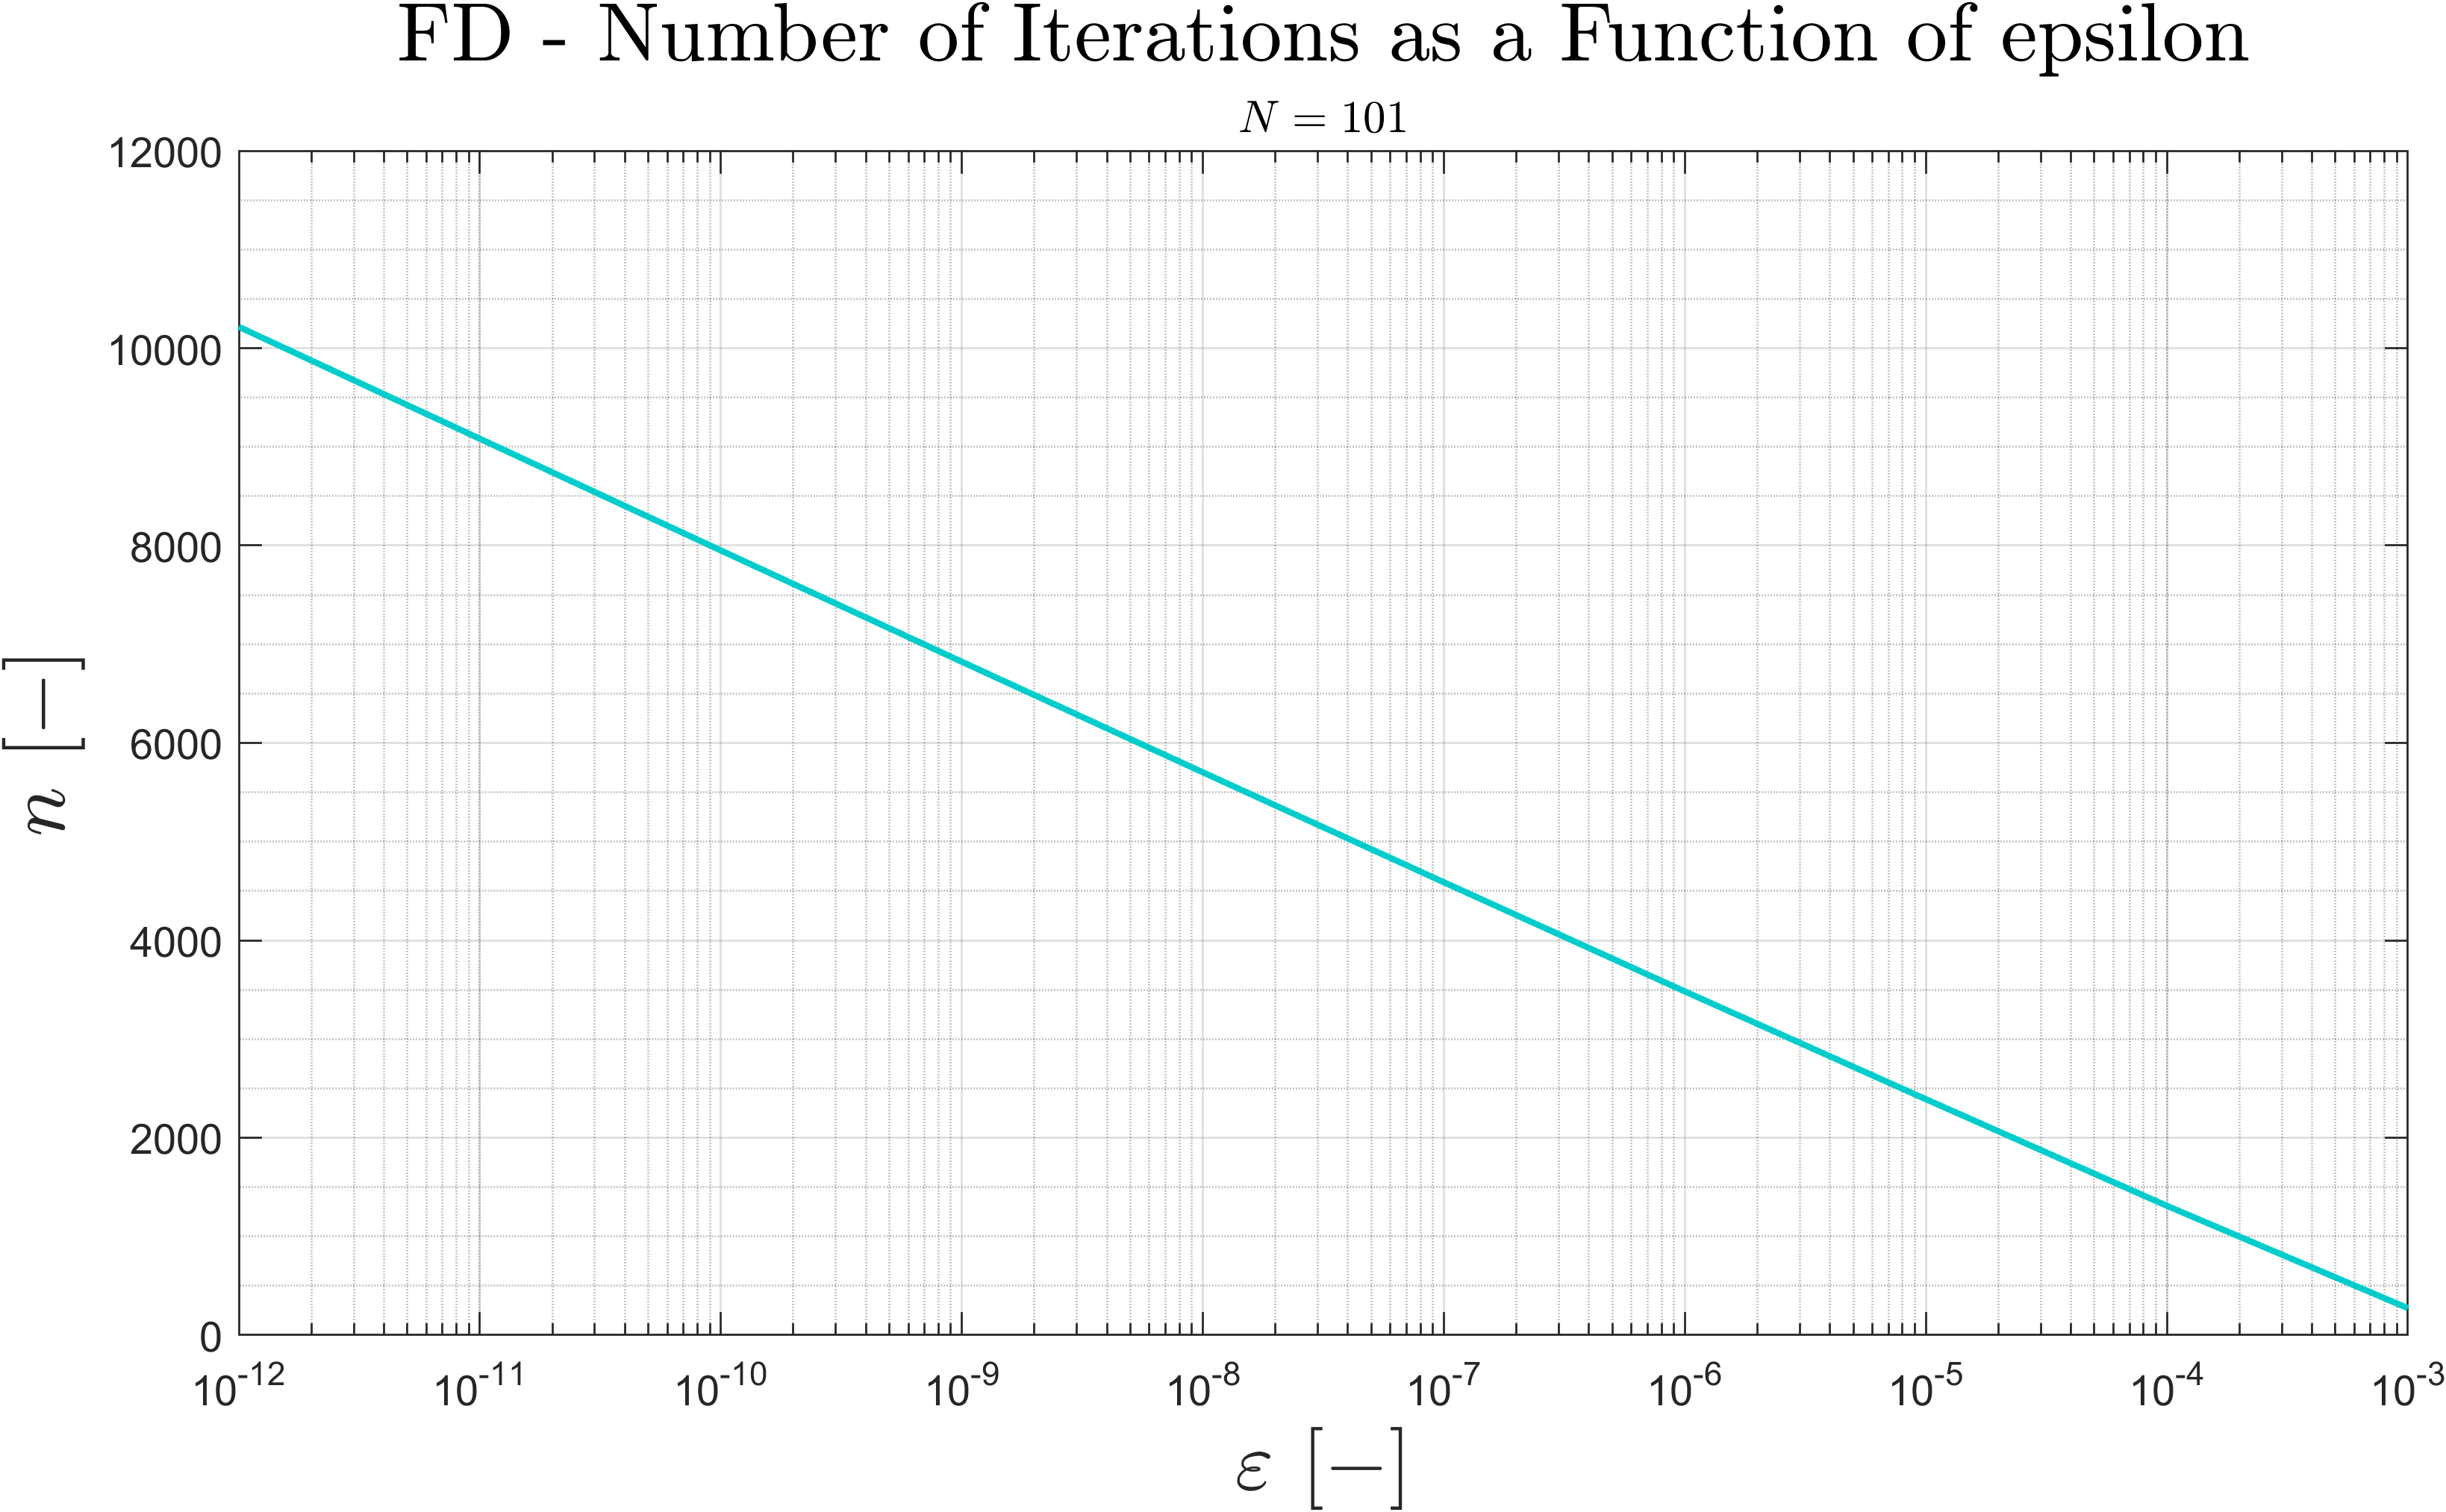
\includegraphics[width=\textwidth]{images/FD - n vs epsilon.png}
        \caption{Number of iterations as a function of epsilon}
        \label{fig: FD - n vs epsilon}
    \end{subfigure}
    \caption{FD - Influence of the convergence criteria $\varepsilon$}
    \label{fig: FD - Influence of epsilon}
\end{figure}
From Fig.\ref{fig: FD - T vs zeta for diff epsilon} we can conclude that for a convergence criteria smaller than $1e^{-8}$, the solution stays the same. From Fig.\ref{fig: FD - n vs epsilon} we can determine that the number of iterations grows exponentially with the decrease of $\varepsilon$. With this two insights at hand, we can determine that $\varepsilon=1e^{-12}$ is a good choice (although it is not economical with the number of iterations).

\subsection{Shooting Method}
\subsubsection{Influence of number of elements N}
\begin{figure}[H]
    \centering
    \begin{subfigure}[c]{0.49\textwidth}
        \centering
        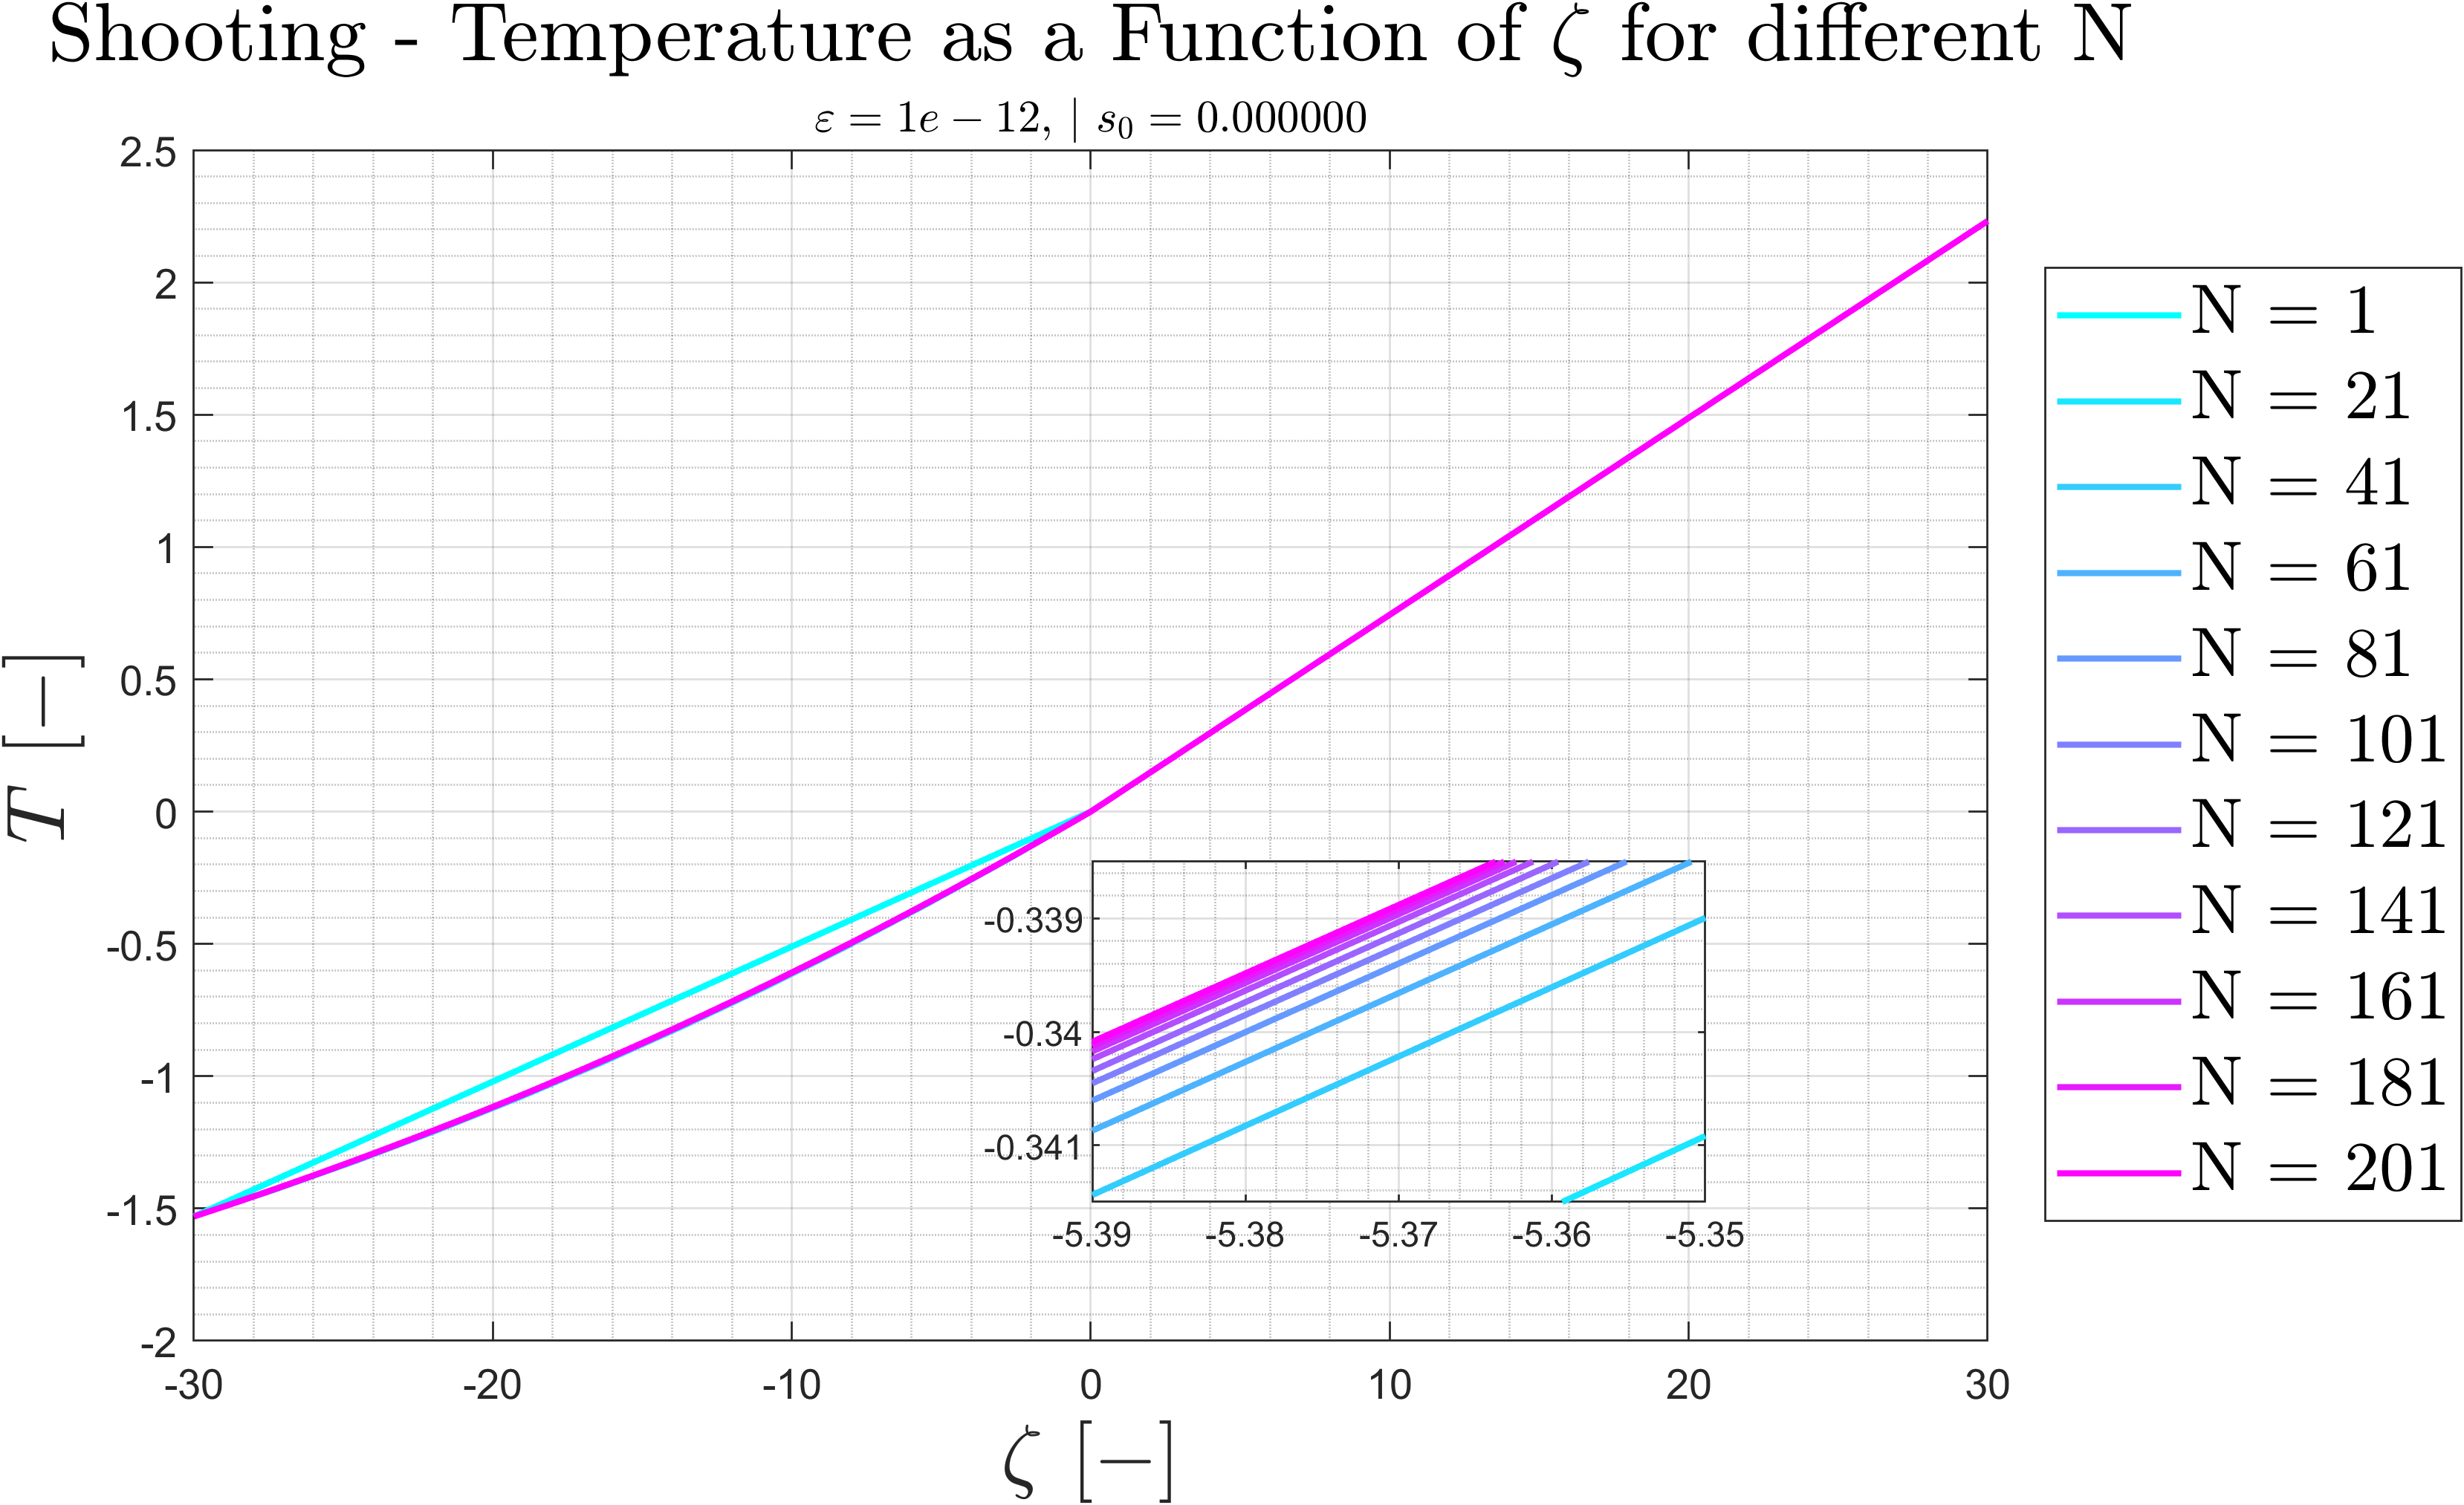
\includegraphics[width=\textwidth]{images/shooting - T vs zeta for diff N.png}
        \caption{Temperature as a Function of $\zeta$ for different N}
        \label{fig: shooting - T vs zeta for diff N}
    \end{subfigure}
    \hfill
    \begin{subfigure}[c]{0.49\textwidth}
        \centering
        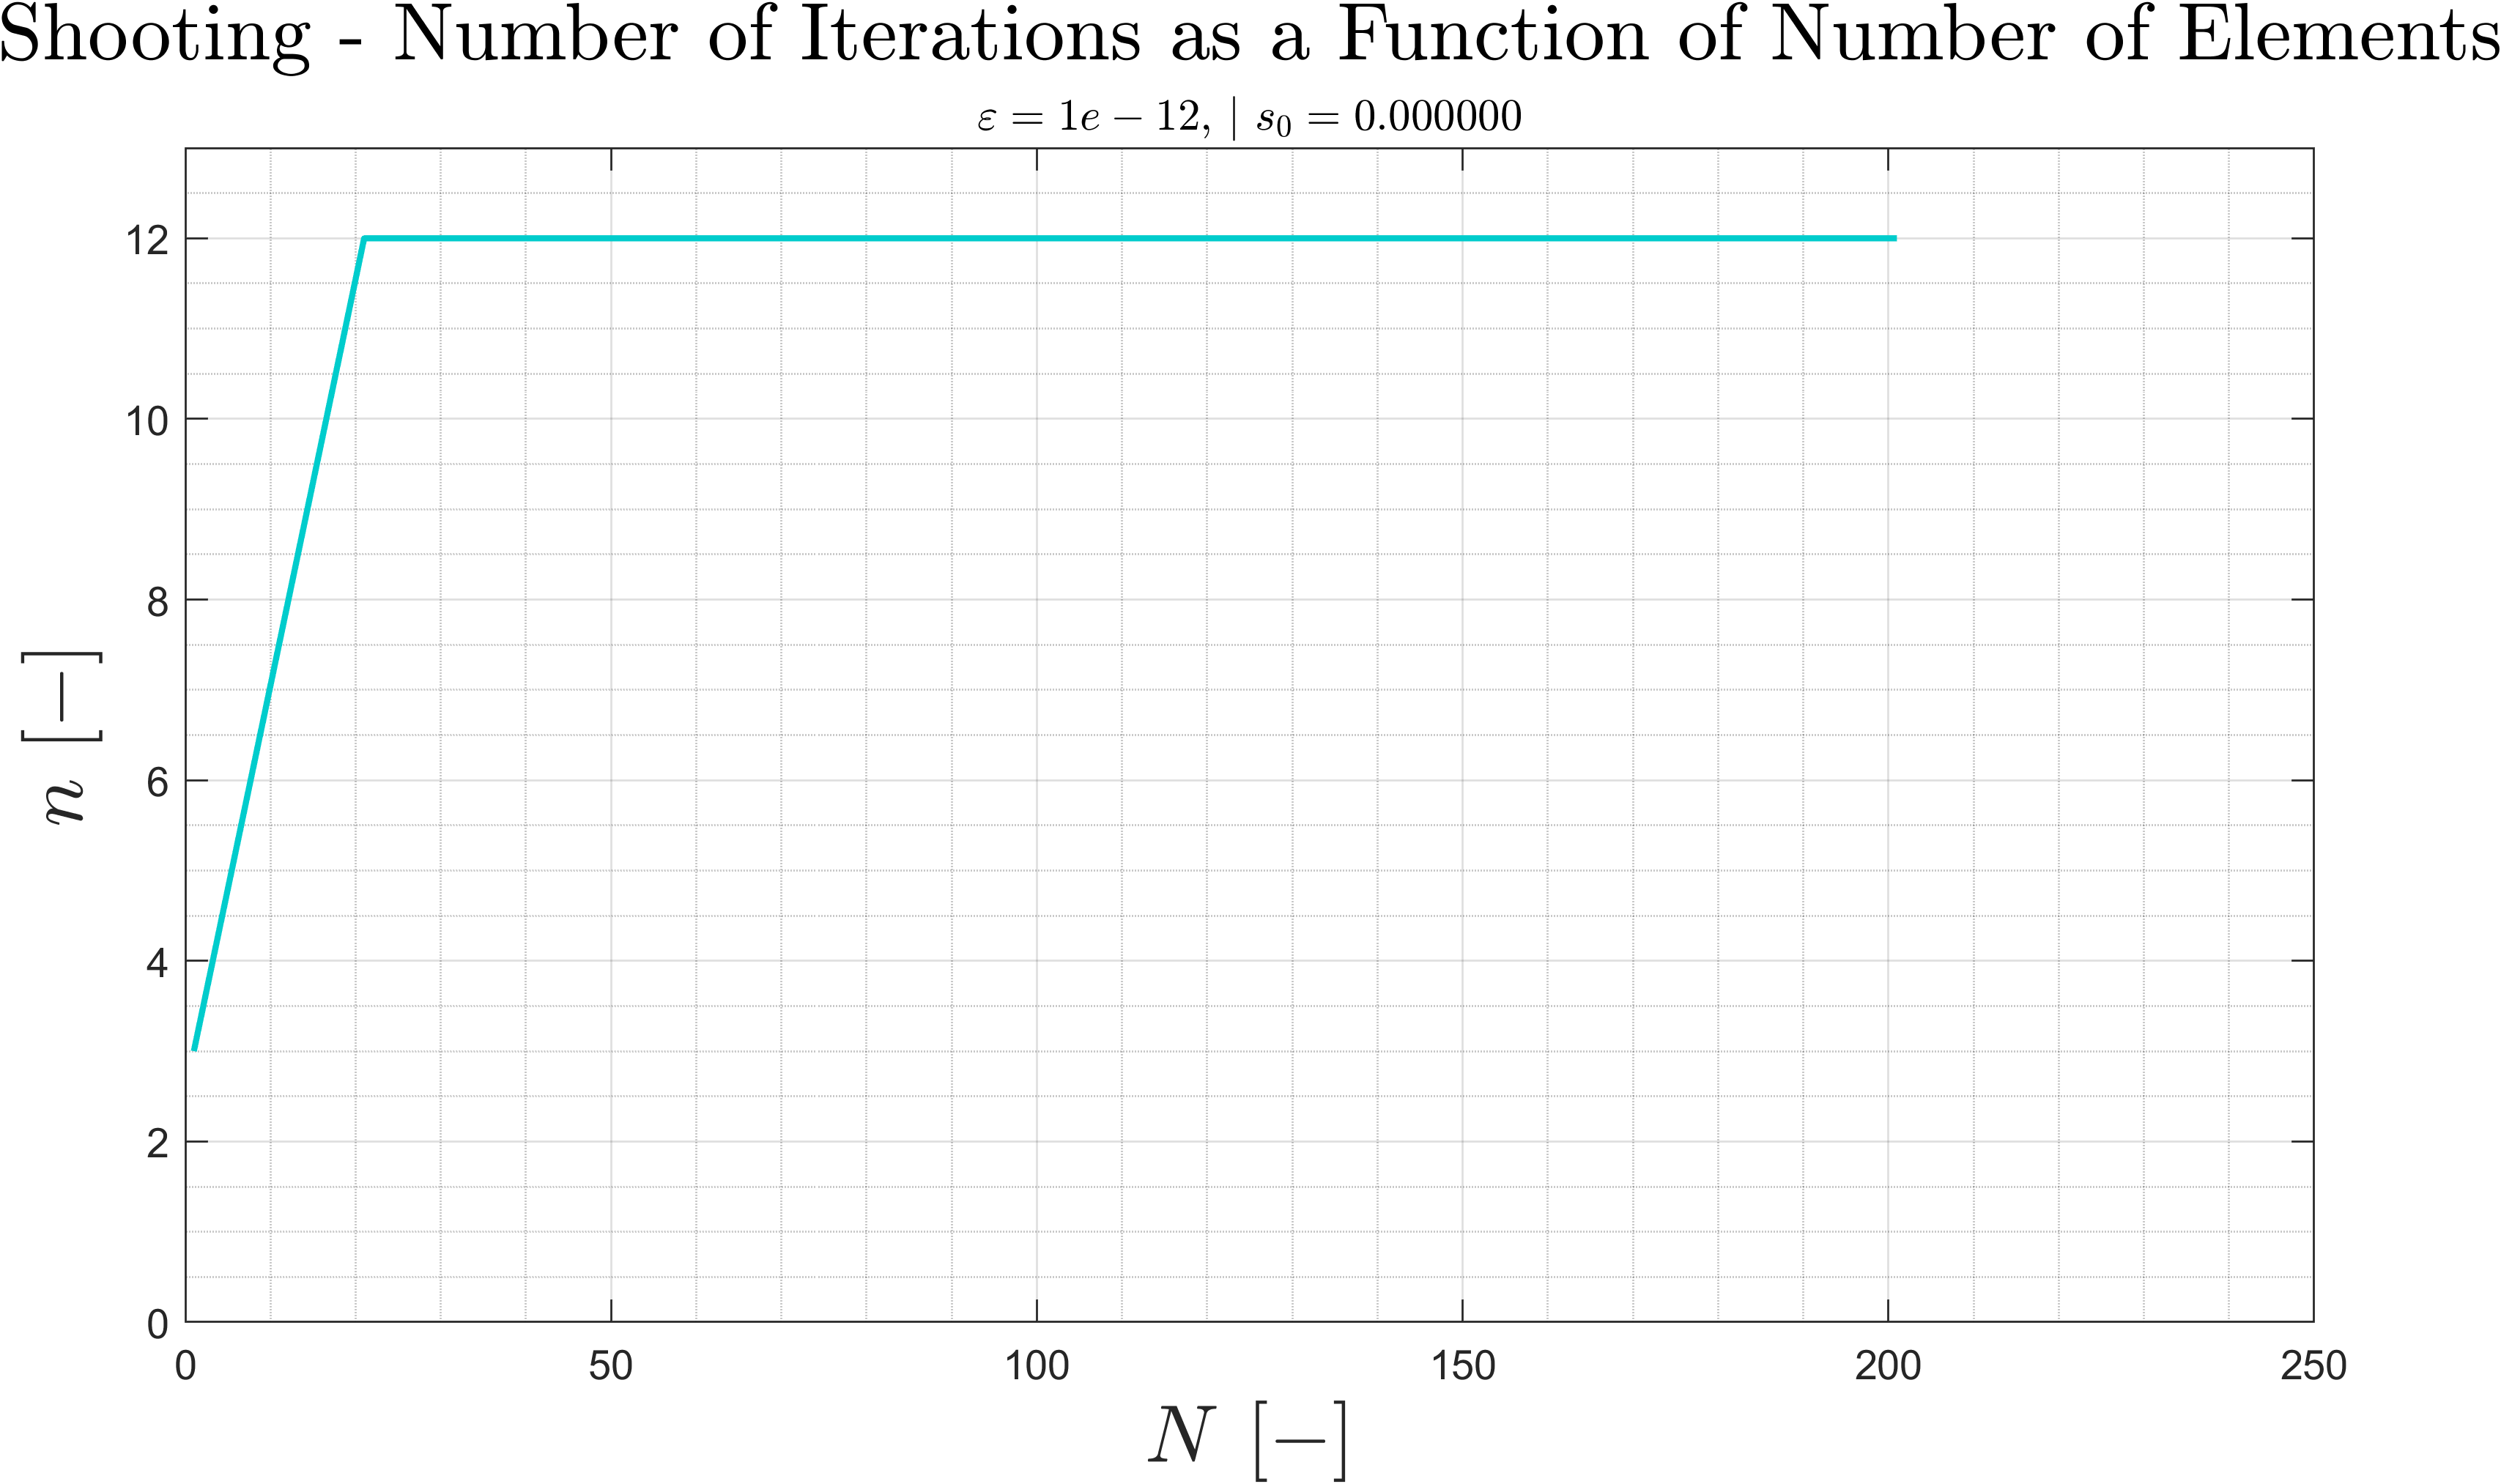
\includegraphics[width=\textwidth]{images/shooting - n vs N.png}
        \caption{Number of iterations as a function of N}
        \label{fig: shooting - n vs N}
    \end{subfigure}
    \caption{Shooting - Influence of the number of elements N}
    \label{fig: shooting - Influence of N}
\end{figure}
In Fig.\ref{fig: shooting - T vs zeta for diff N} we can see that for N bigger than 100, the solution does not really change. From Fig.\ref{fig: shooting - n vs N} we can see that for more than 25 elements, the number of iterations stays constant for a certain convergence criteria and initial condition. We can conclude that $N=101$ is a sufficient number of elements.

\subsubsection{Influence of convergence criteria $\varepsilon$}
\begin{figure}[H]
    \centering
    \begin{subfigure}[c]{0.49\textwidth}
        \centering
        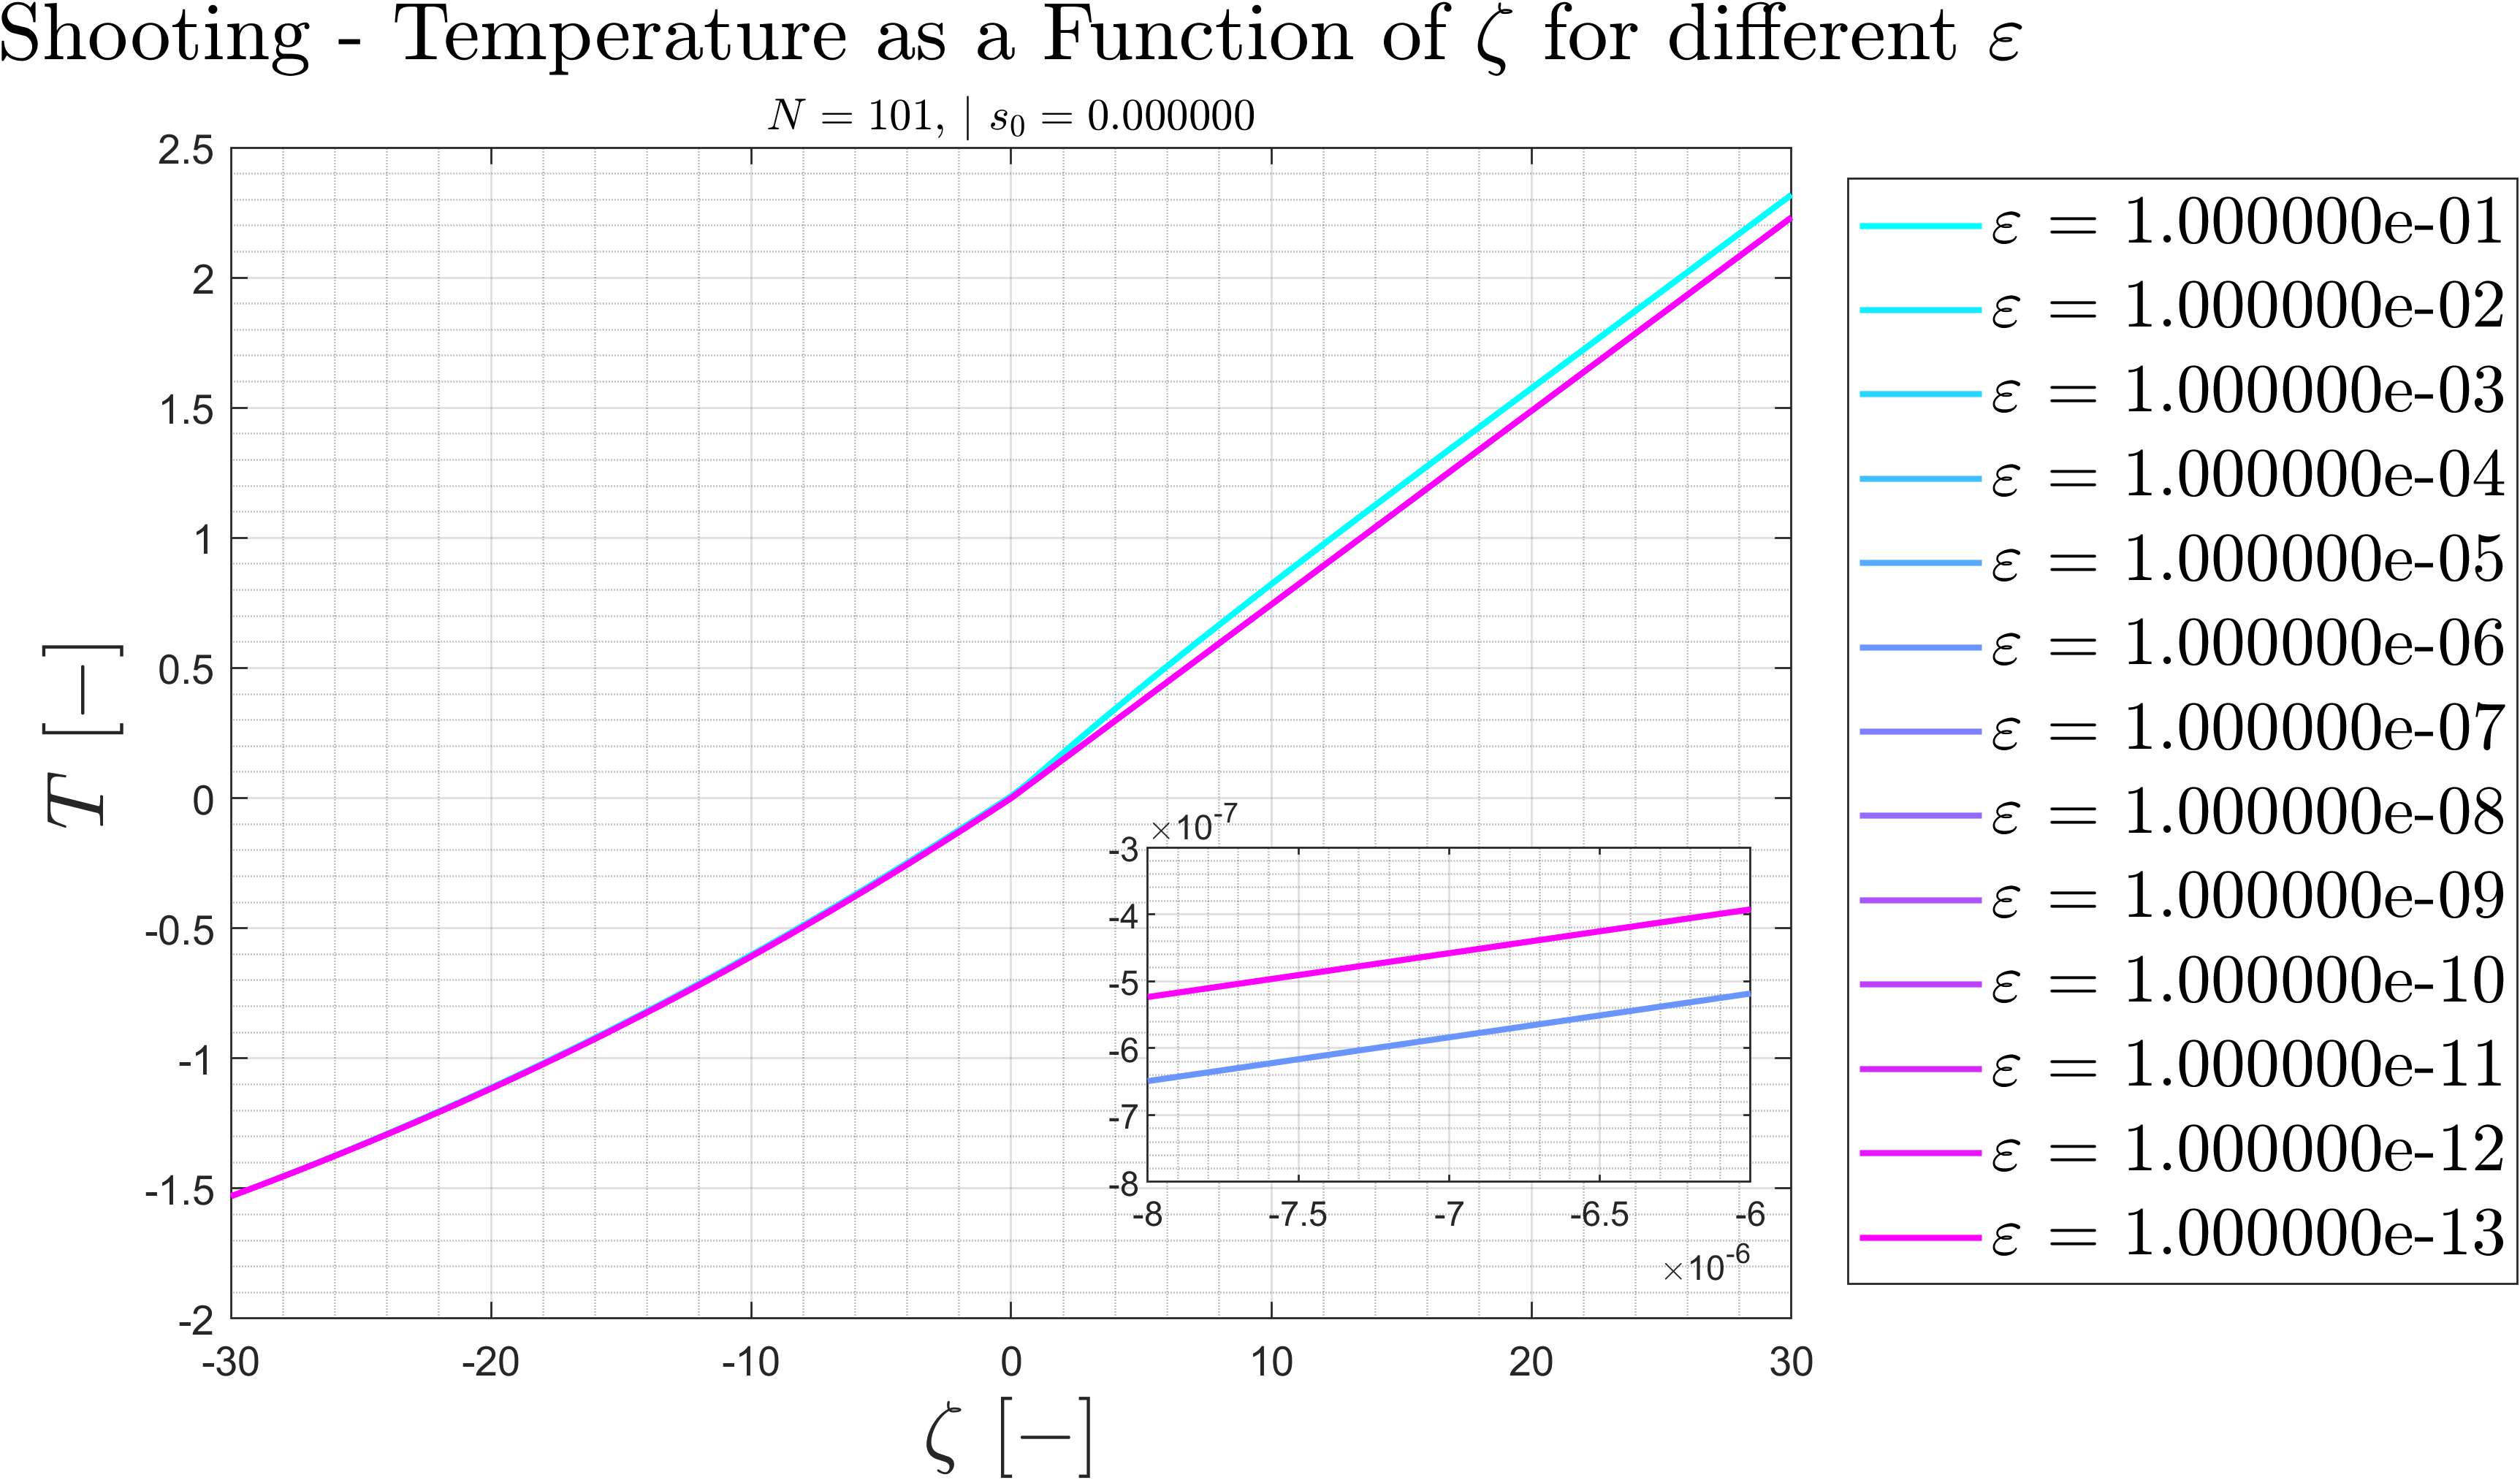
\includegraphics[width=\textwidth]{images/shooting - T vs zeta for diff epsilon.png}
        \caption{Temperature as a Function of $\zeta$ for different $\varepsilon$}
        \label{fig: shooting - T vs zeta for diff epsilon}
    \end{subfigure}
    \hfill
    \begin{subfigure}[c]{0.49\textwidth}
        \centering
        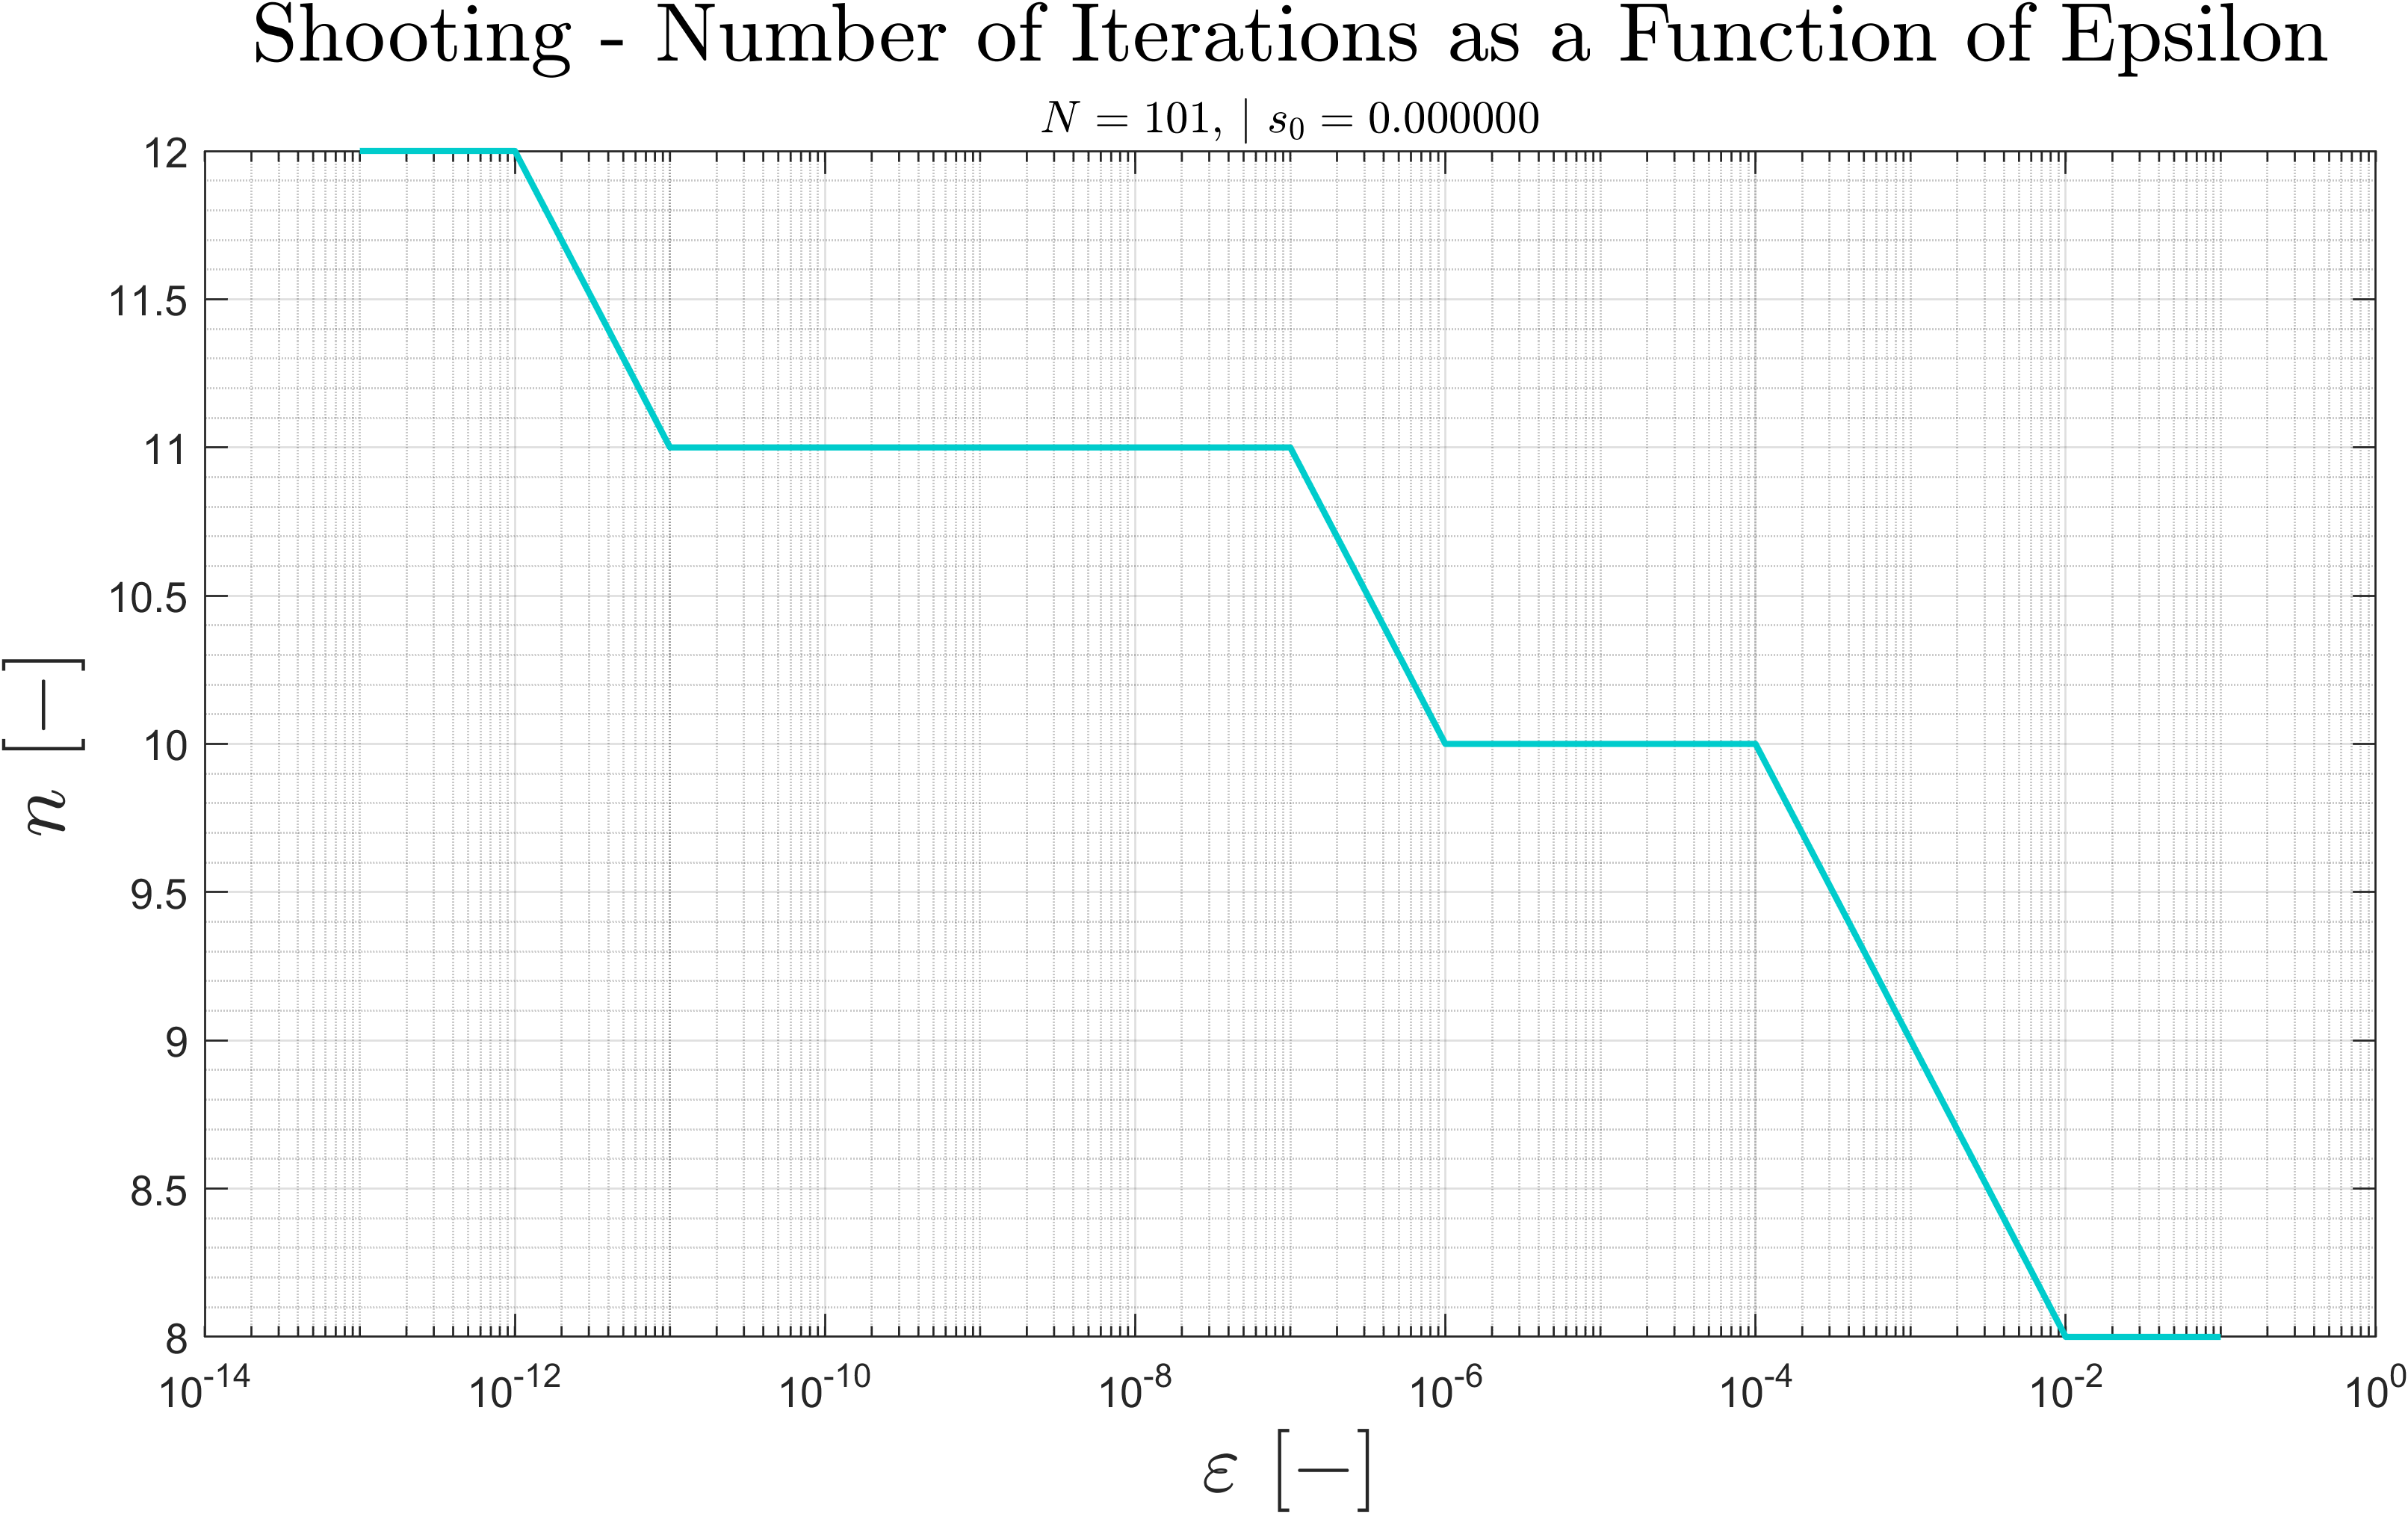
\includegraphics[width=\textwidth]{images/shooting - n vs epsilon.png}
        \caption{Number of iterations as a function of epsilon}
        \label{fig: shooting - n vs epsilon}
    \end{subfigure}
    \caption{Shooting - Influence of the convergence criteria $\varepsilon$}
    \label{fig: shooting - Influence of epsilon}
\end{figure}
Figure \ref{fig: shooting - T vs zeta for diff epsilon} shows that for a convergence criteria smaller than $1e^{-6}$, the differences between the solutions are because of rounding errors. From Fig.\ref{fig: shooting - n vs epsilon} we can learn that the number of iterations does not change much for Different convergence criteria. We can determine that $\varepsilon=1e^{-12}$ is a good choice.

\subsubsection{Influence of initial guess $s_0$}
\begin{figure}[H]
    \centering
    \begin{subfigure}[c]{0.49\textwidth}
        \centering
        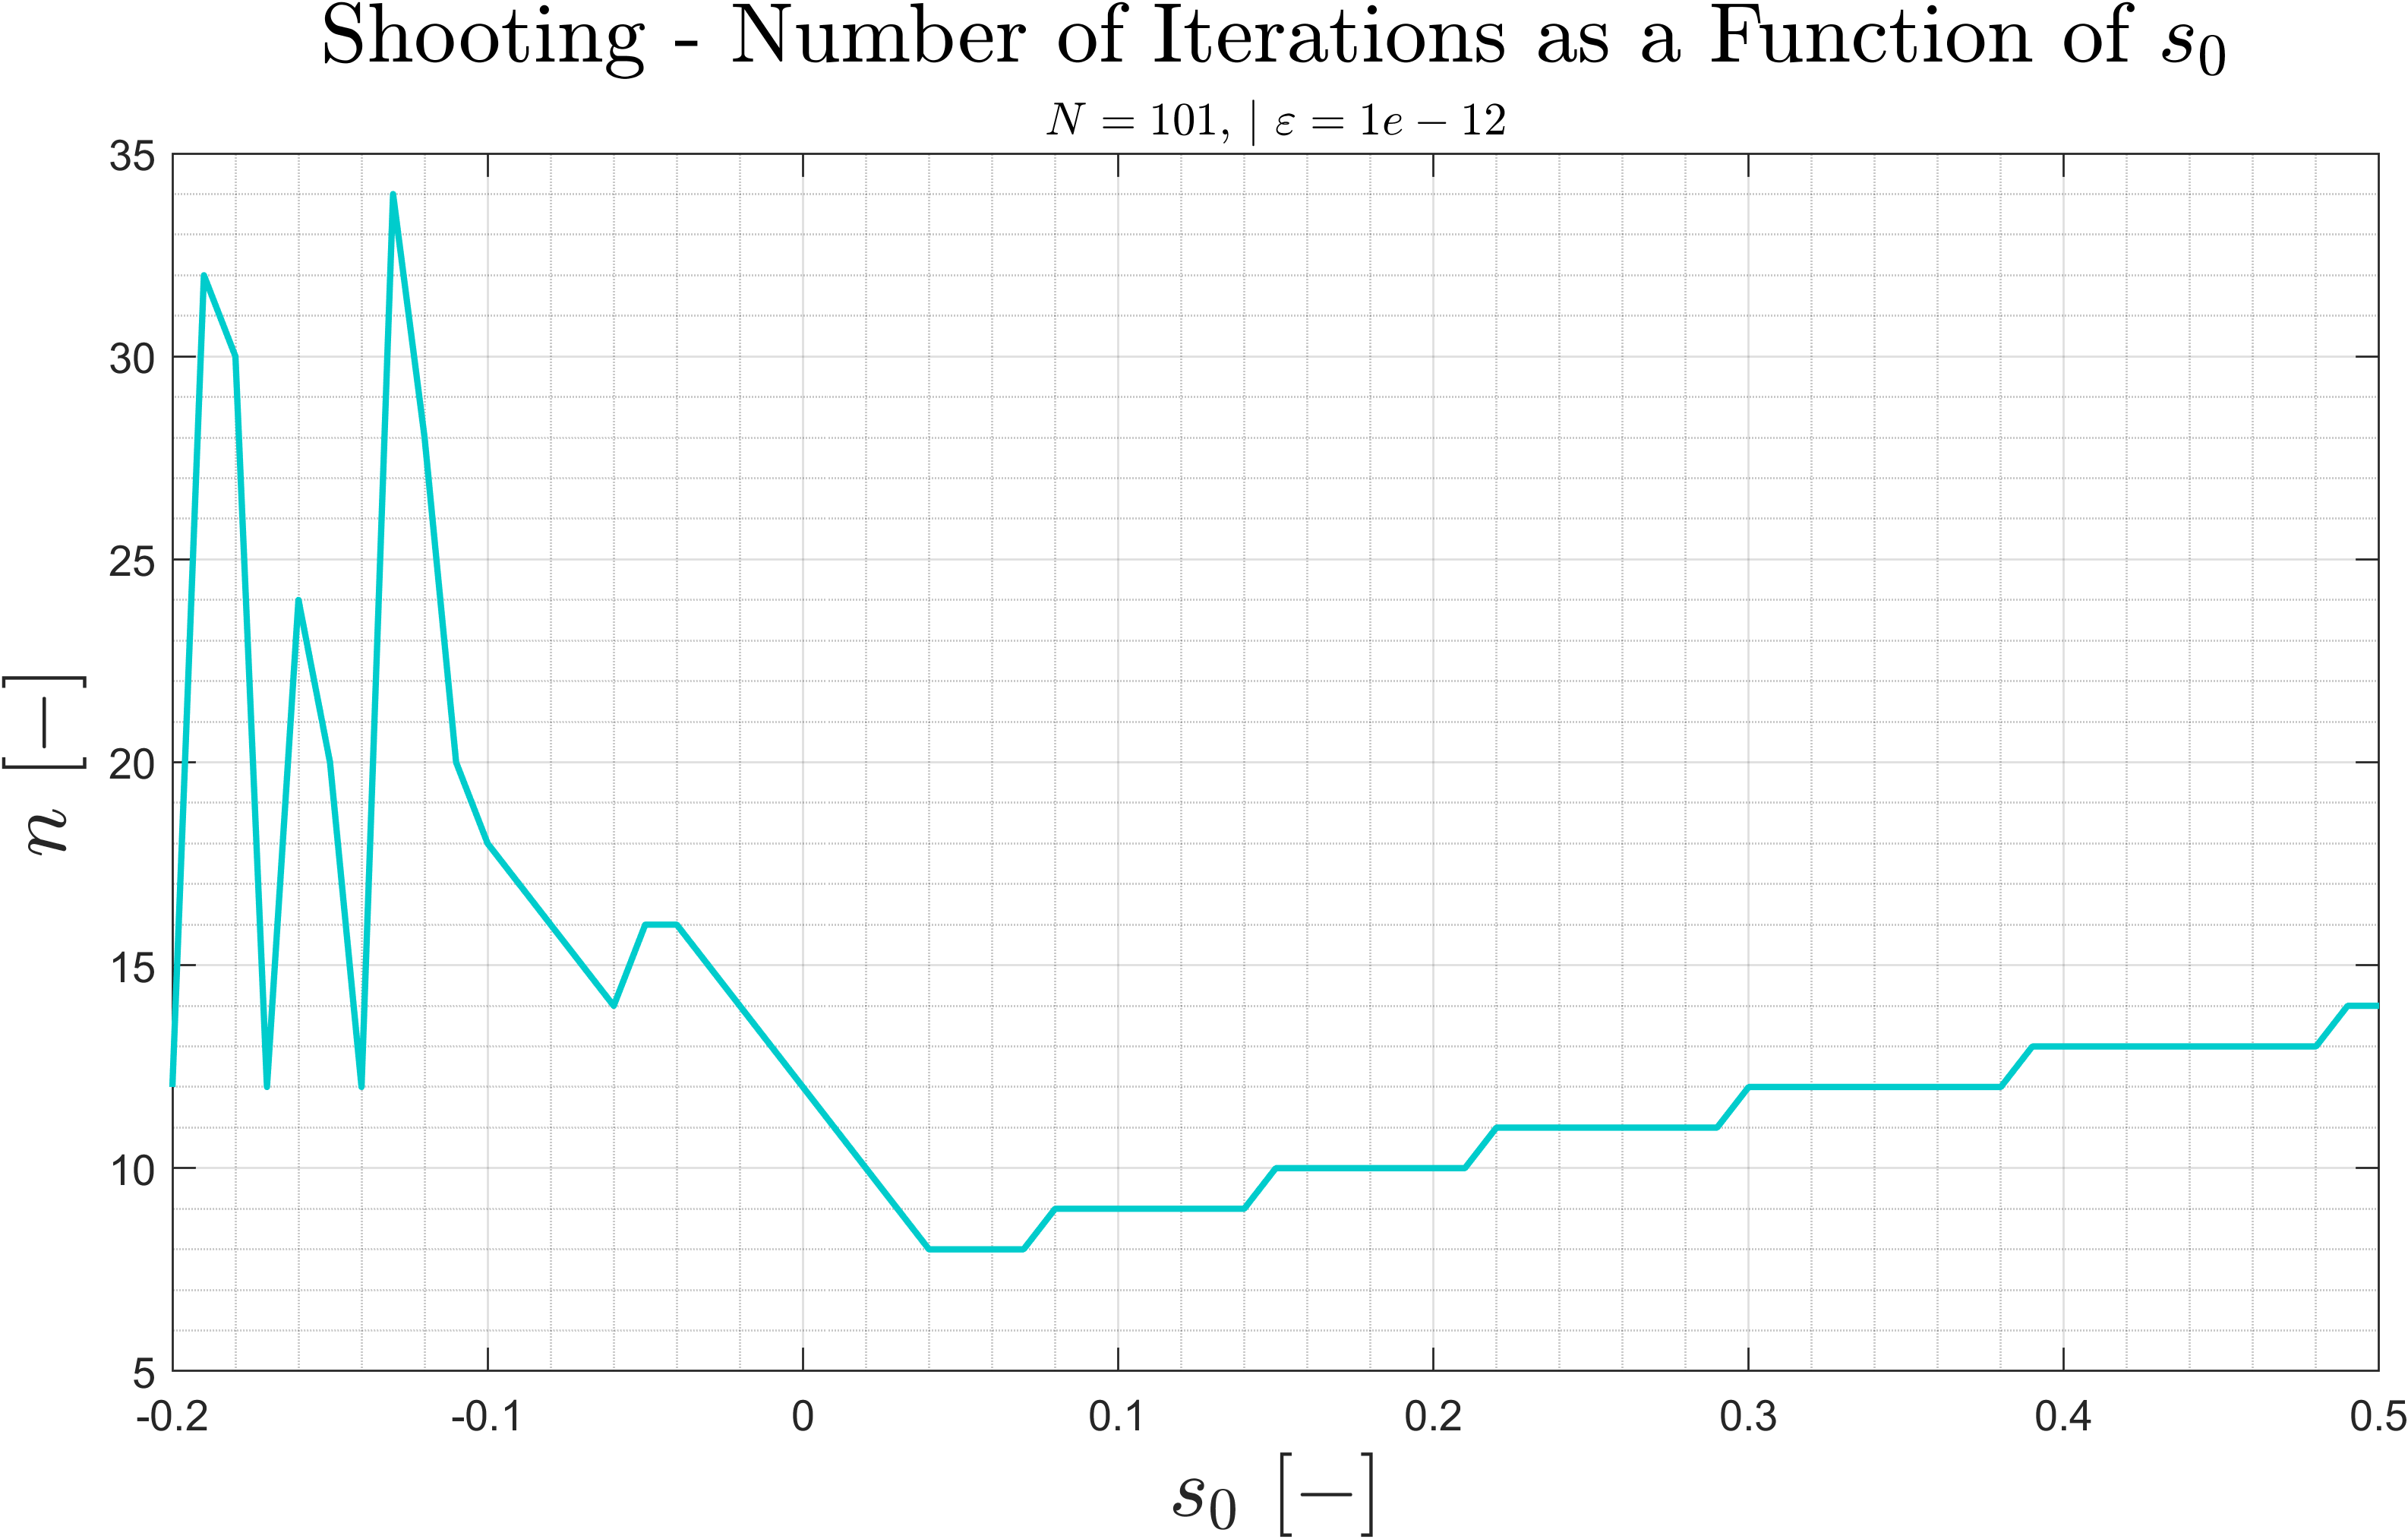
\includegraphics[width=\textwidth]{images/shooting - n vs s0 - with negative.png}
        \caption{}
        \label{fig: shooting - n vs s0 - with negative}
    \end{subfigure}
    \hfill
    \begin{subfigure}[c]{0.49\textwidth}
        \centering
        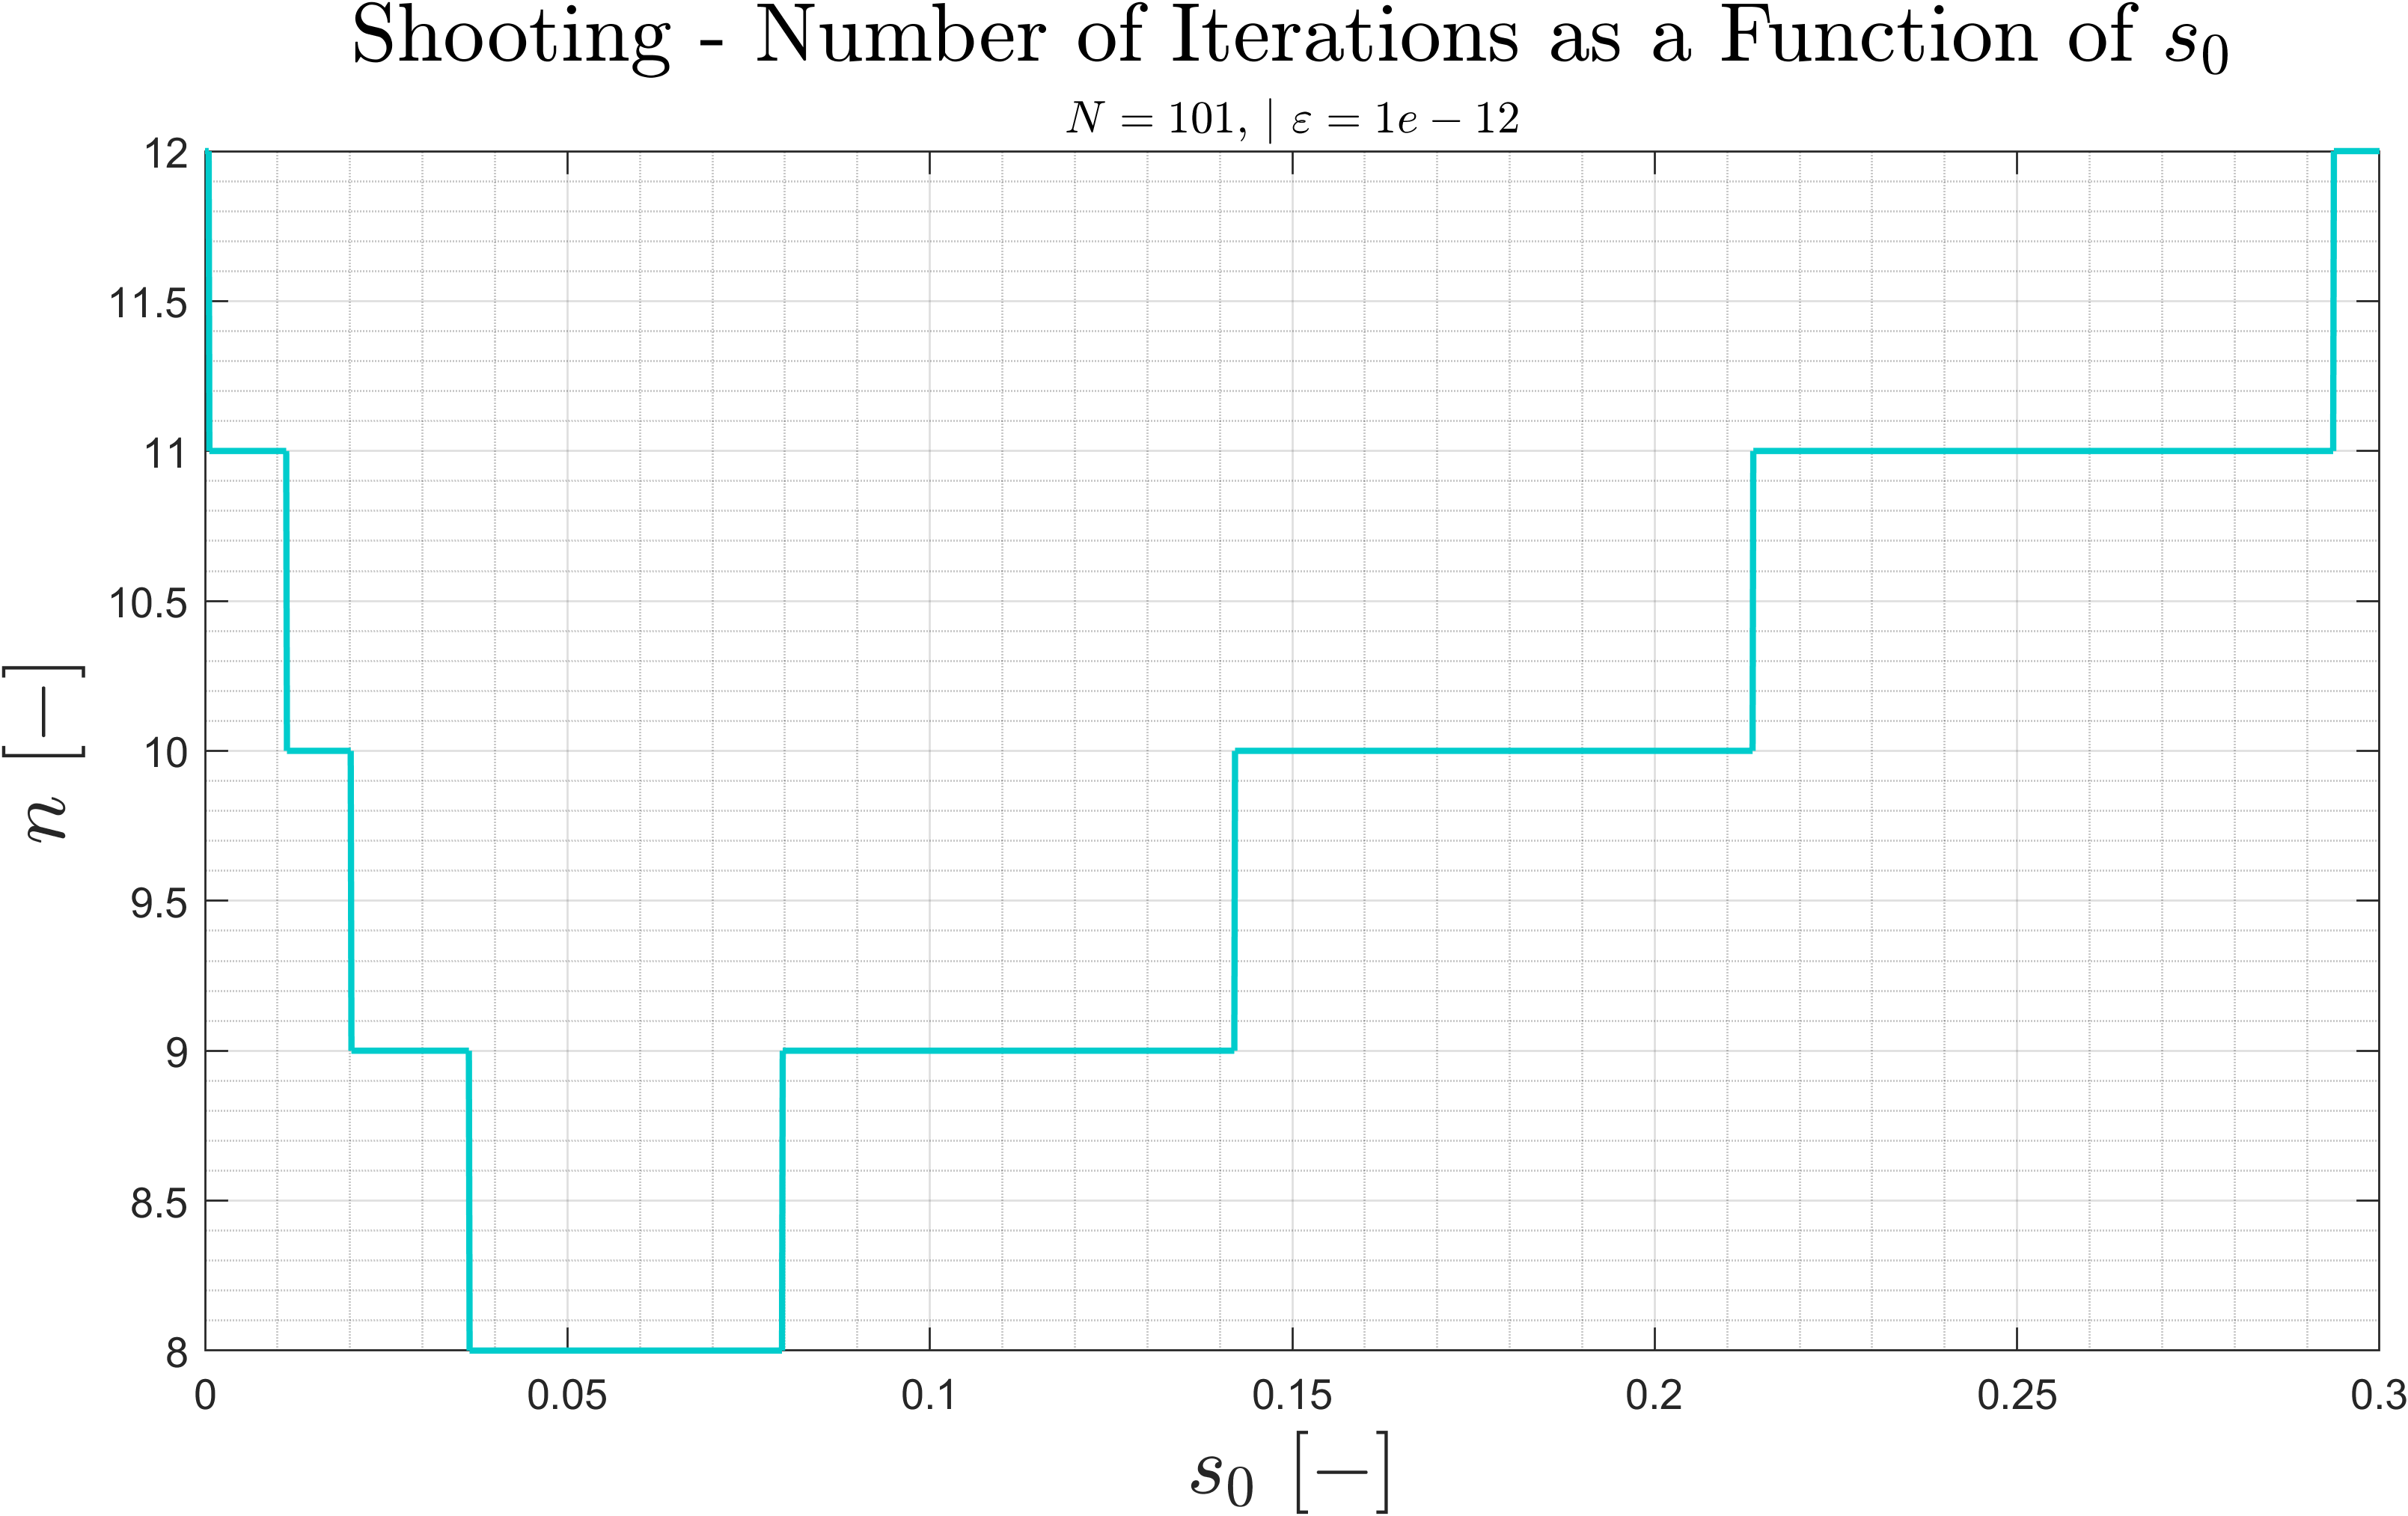
\includegraphics[width=\textwidth]{images/shooting - n vs s0 - no negative.png}
        \caption{}
        \label{fig: shooting - n vs s0 - no negative}
    \end{subfigure}
    \caption{Number of iterations as a function of initial guess}
    \label{fig: shooting - Influence of s0}
\end{figure}
Figure \ref{fig: shooting - Influence of s0} shows that for different negative initial conditions, the number of iterations is not stable. Moreover, we can learn that the real initial slope is around 0.05, as this is the condition for which it took the least amount of steps to converge.

\newpage
\section{Results and Discussion}
In the following section, the numerical solution for the ODE will be presented using the parameters chosen in the previous section (Sec.\ref{sec: Influence of The Numerical Methods}).
\begin{figure}[H]
    \centering
    \begin{subfigure}[c]{0.49\textwidth}
        \centering
        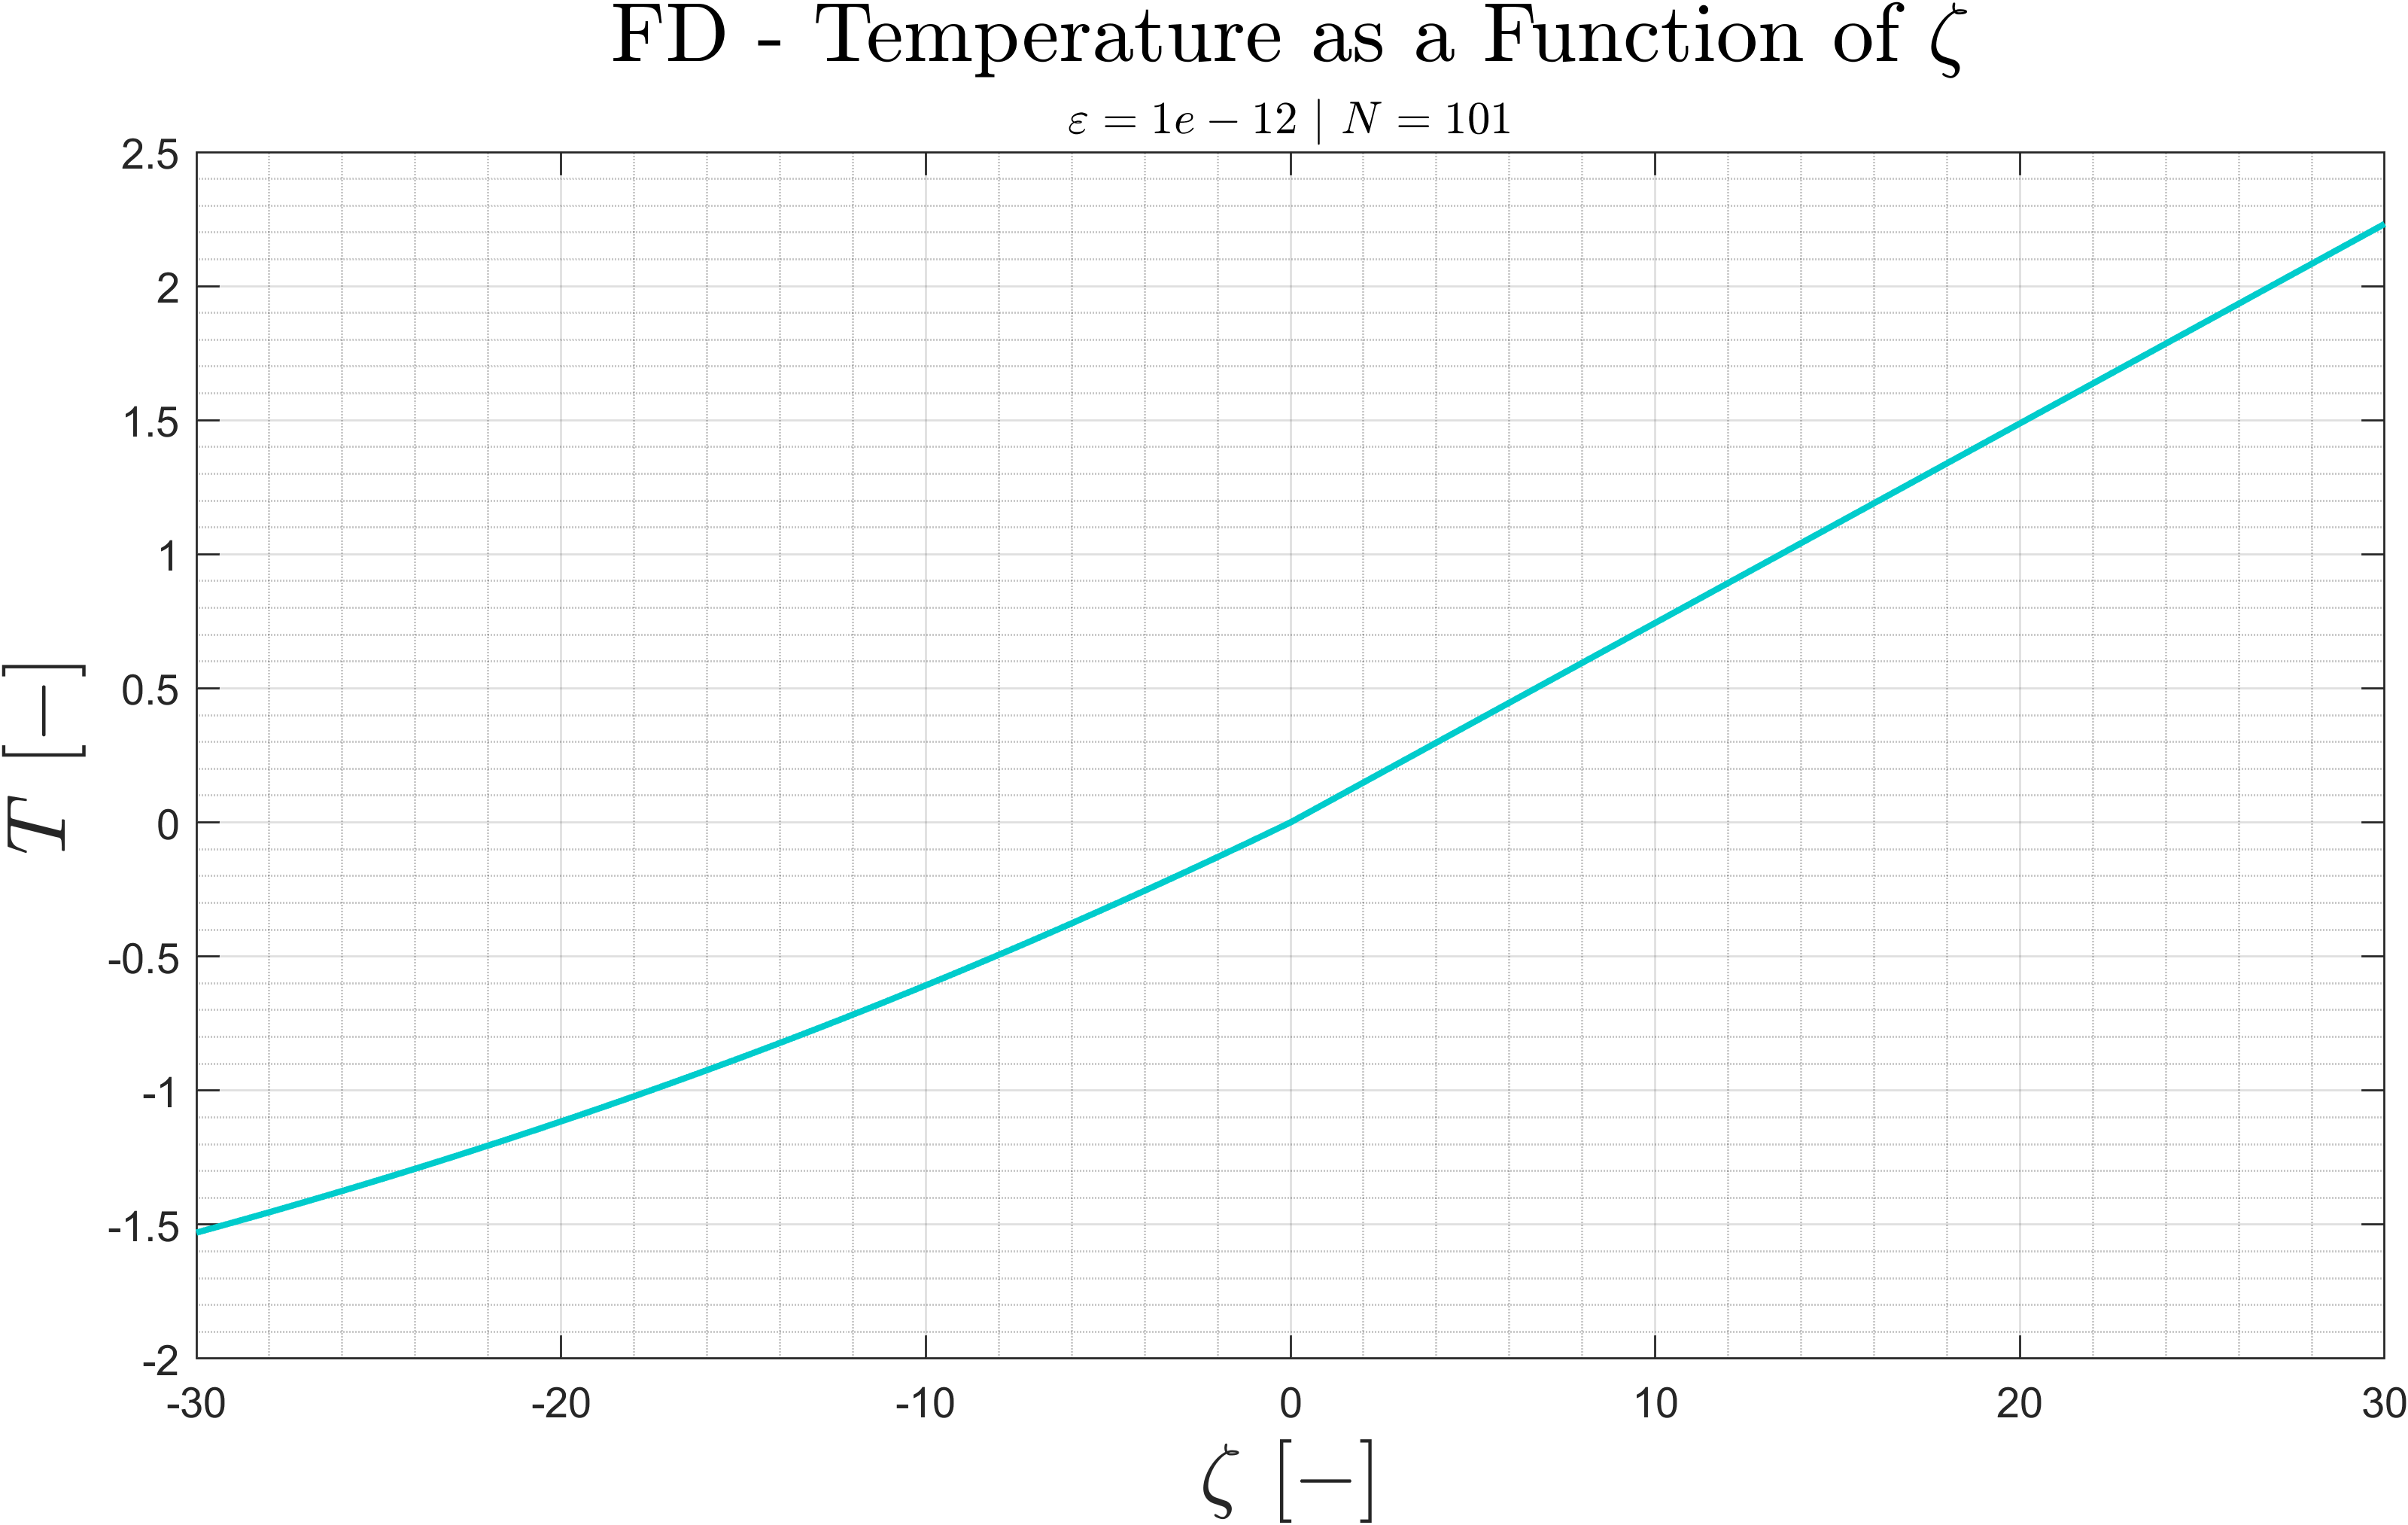
\includegraphics[width=\textwidth]{images/FD - T vs zeta.png}
        \caption{FD - temperature as a function of $\zeta$}
        \label{fig: FD - T vs zeta}
    \end{subfigure}
    \hfill
    \begin{subfigure}[c]{0.49\textwidth}
        \centering
        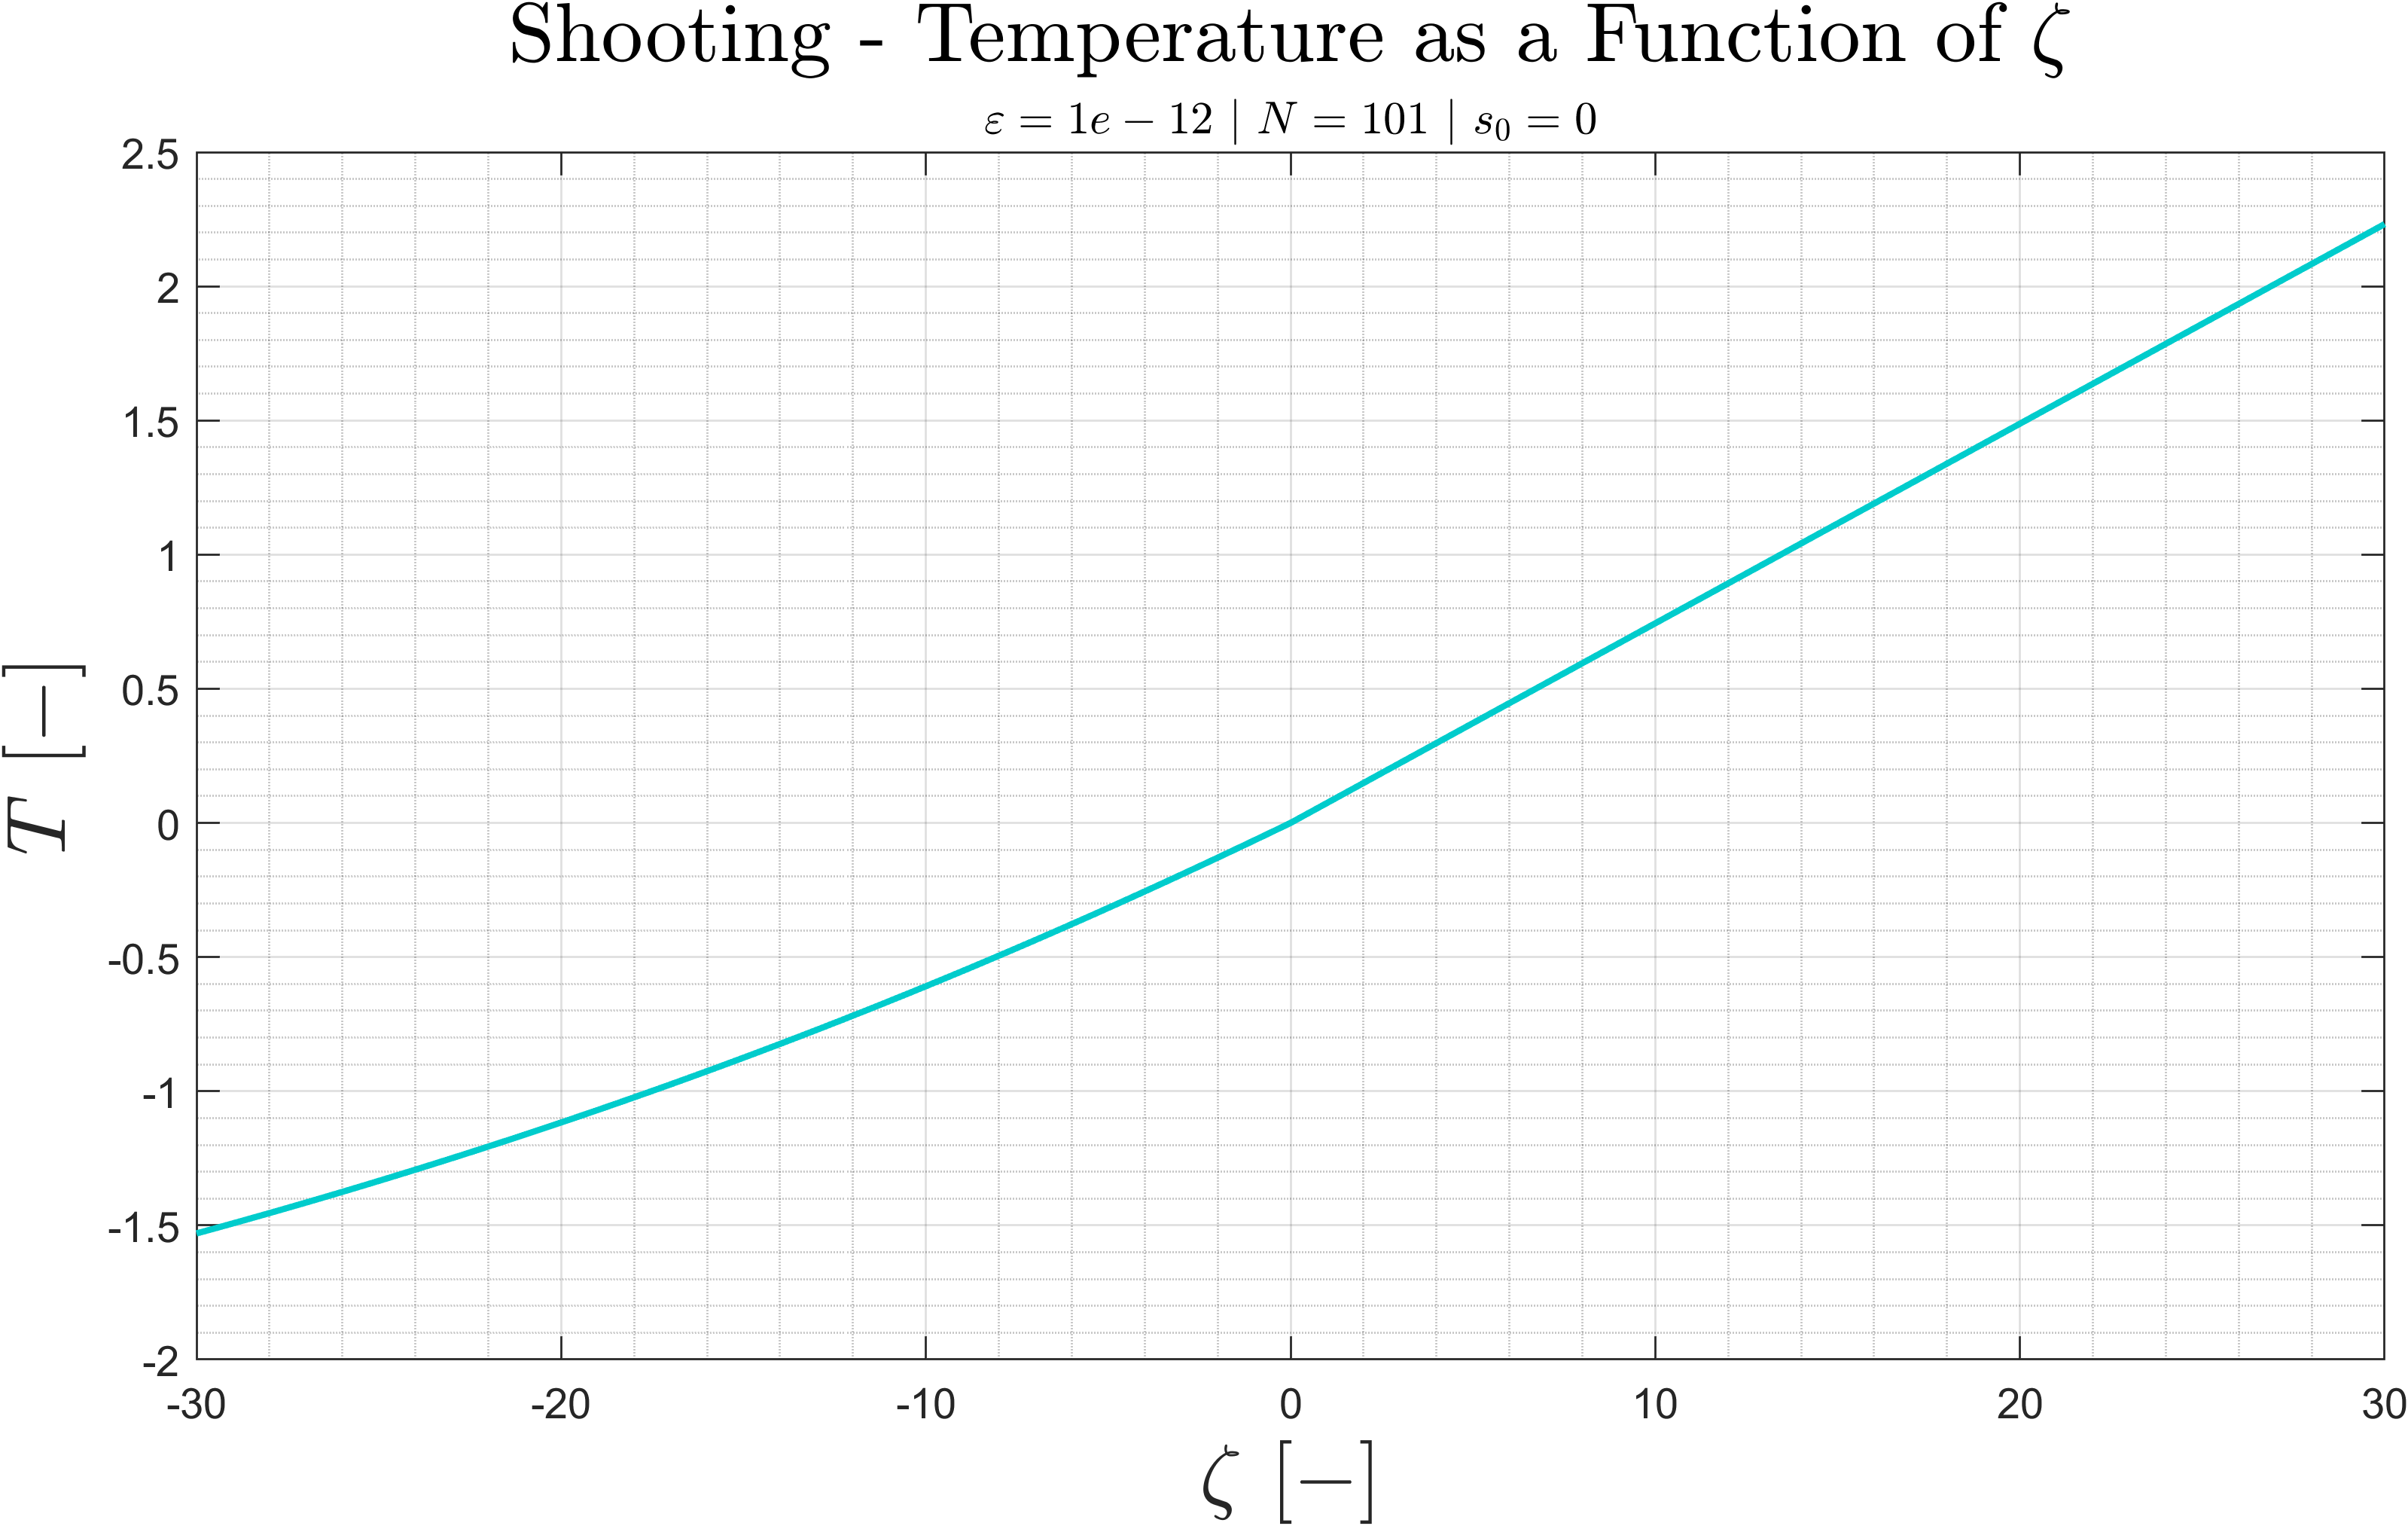
\includegraphics[width=\textwidth]{images/shooting - T vs zeta.png}
        \caption{shooting - temperature as a function of $\zeta$}
        \label{fig: shooting - T vs zeta}
    \end{subfigure}
    \caption{Temperature as a function of $\zeta$}
    \label{fig: T vs zeta}
\end{figure}
\noindent We can see in Fig.\ref{fig: T vs zeta} that there are no differences in the final result between the two methods. With the finite differences method, it took about 10,000 iterations to converge, while with the shooting method, it took only around 10 steps. On the left side of $\zeta=0$, the solution increases monotonically and faster than linearly. On the right side of $\zeta=0$, the solution increases linearly with $\zeta$.
\begin{figure}[H]
    \centering
    \begin{subfigure}[c]{0.49\textwidth}
        \centering
        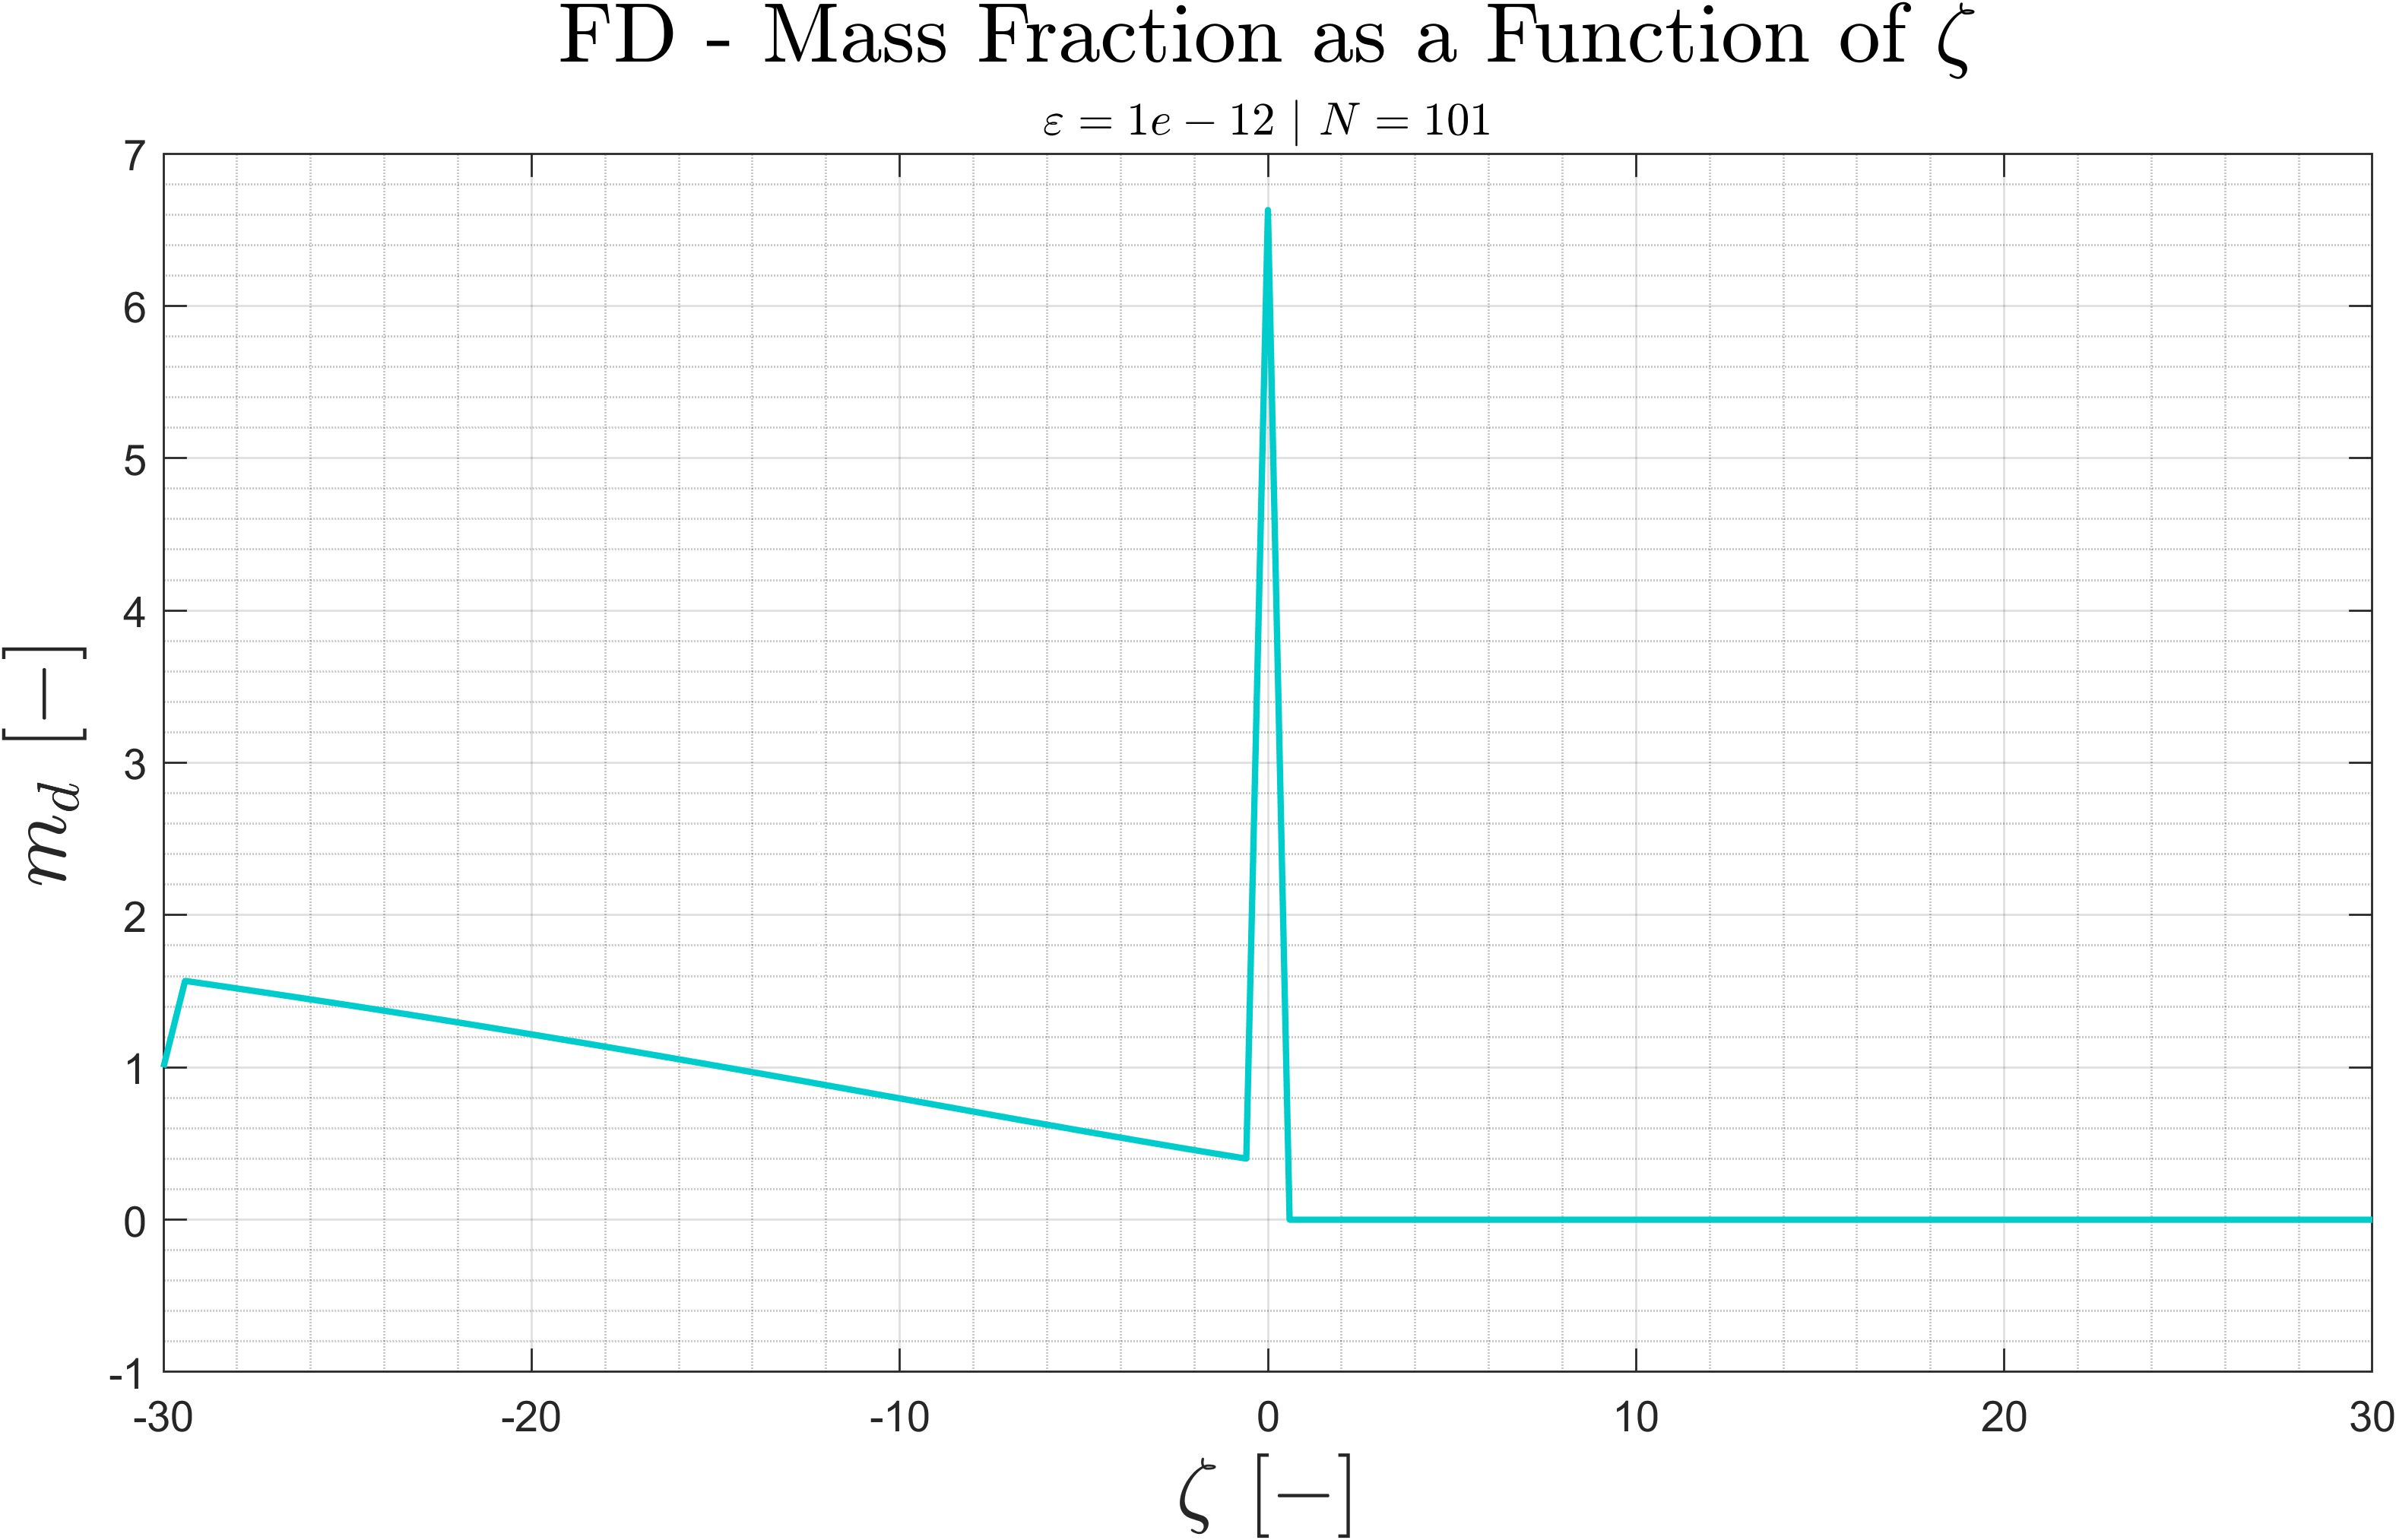
\includegraphics[width=\textwidth]{images/FD - md vs zeta.png}
        \caption{FD - mass fraction as a function of $\zeta$}
        \label{fig: FD - md vs zeta}
    \end{subfigure}
    \hfill
    \begin{subfigure}[c]{0.49\textwidth}
        \centering
        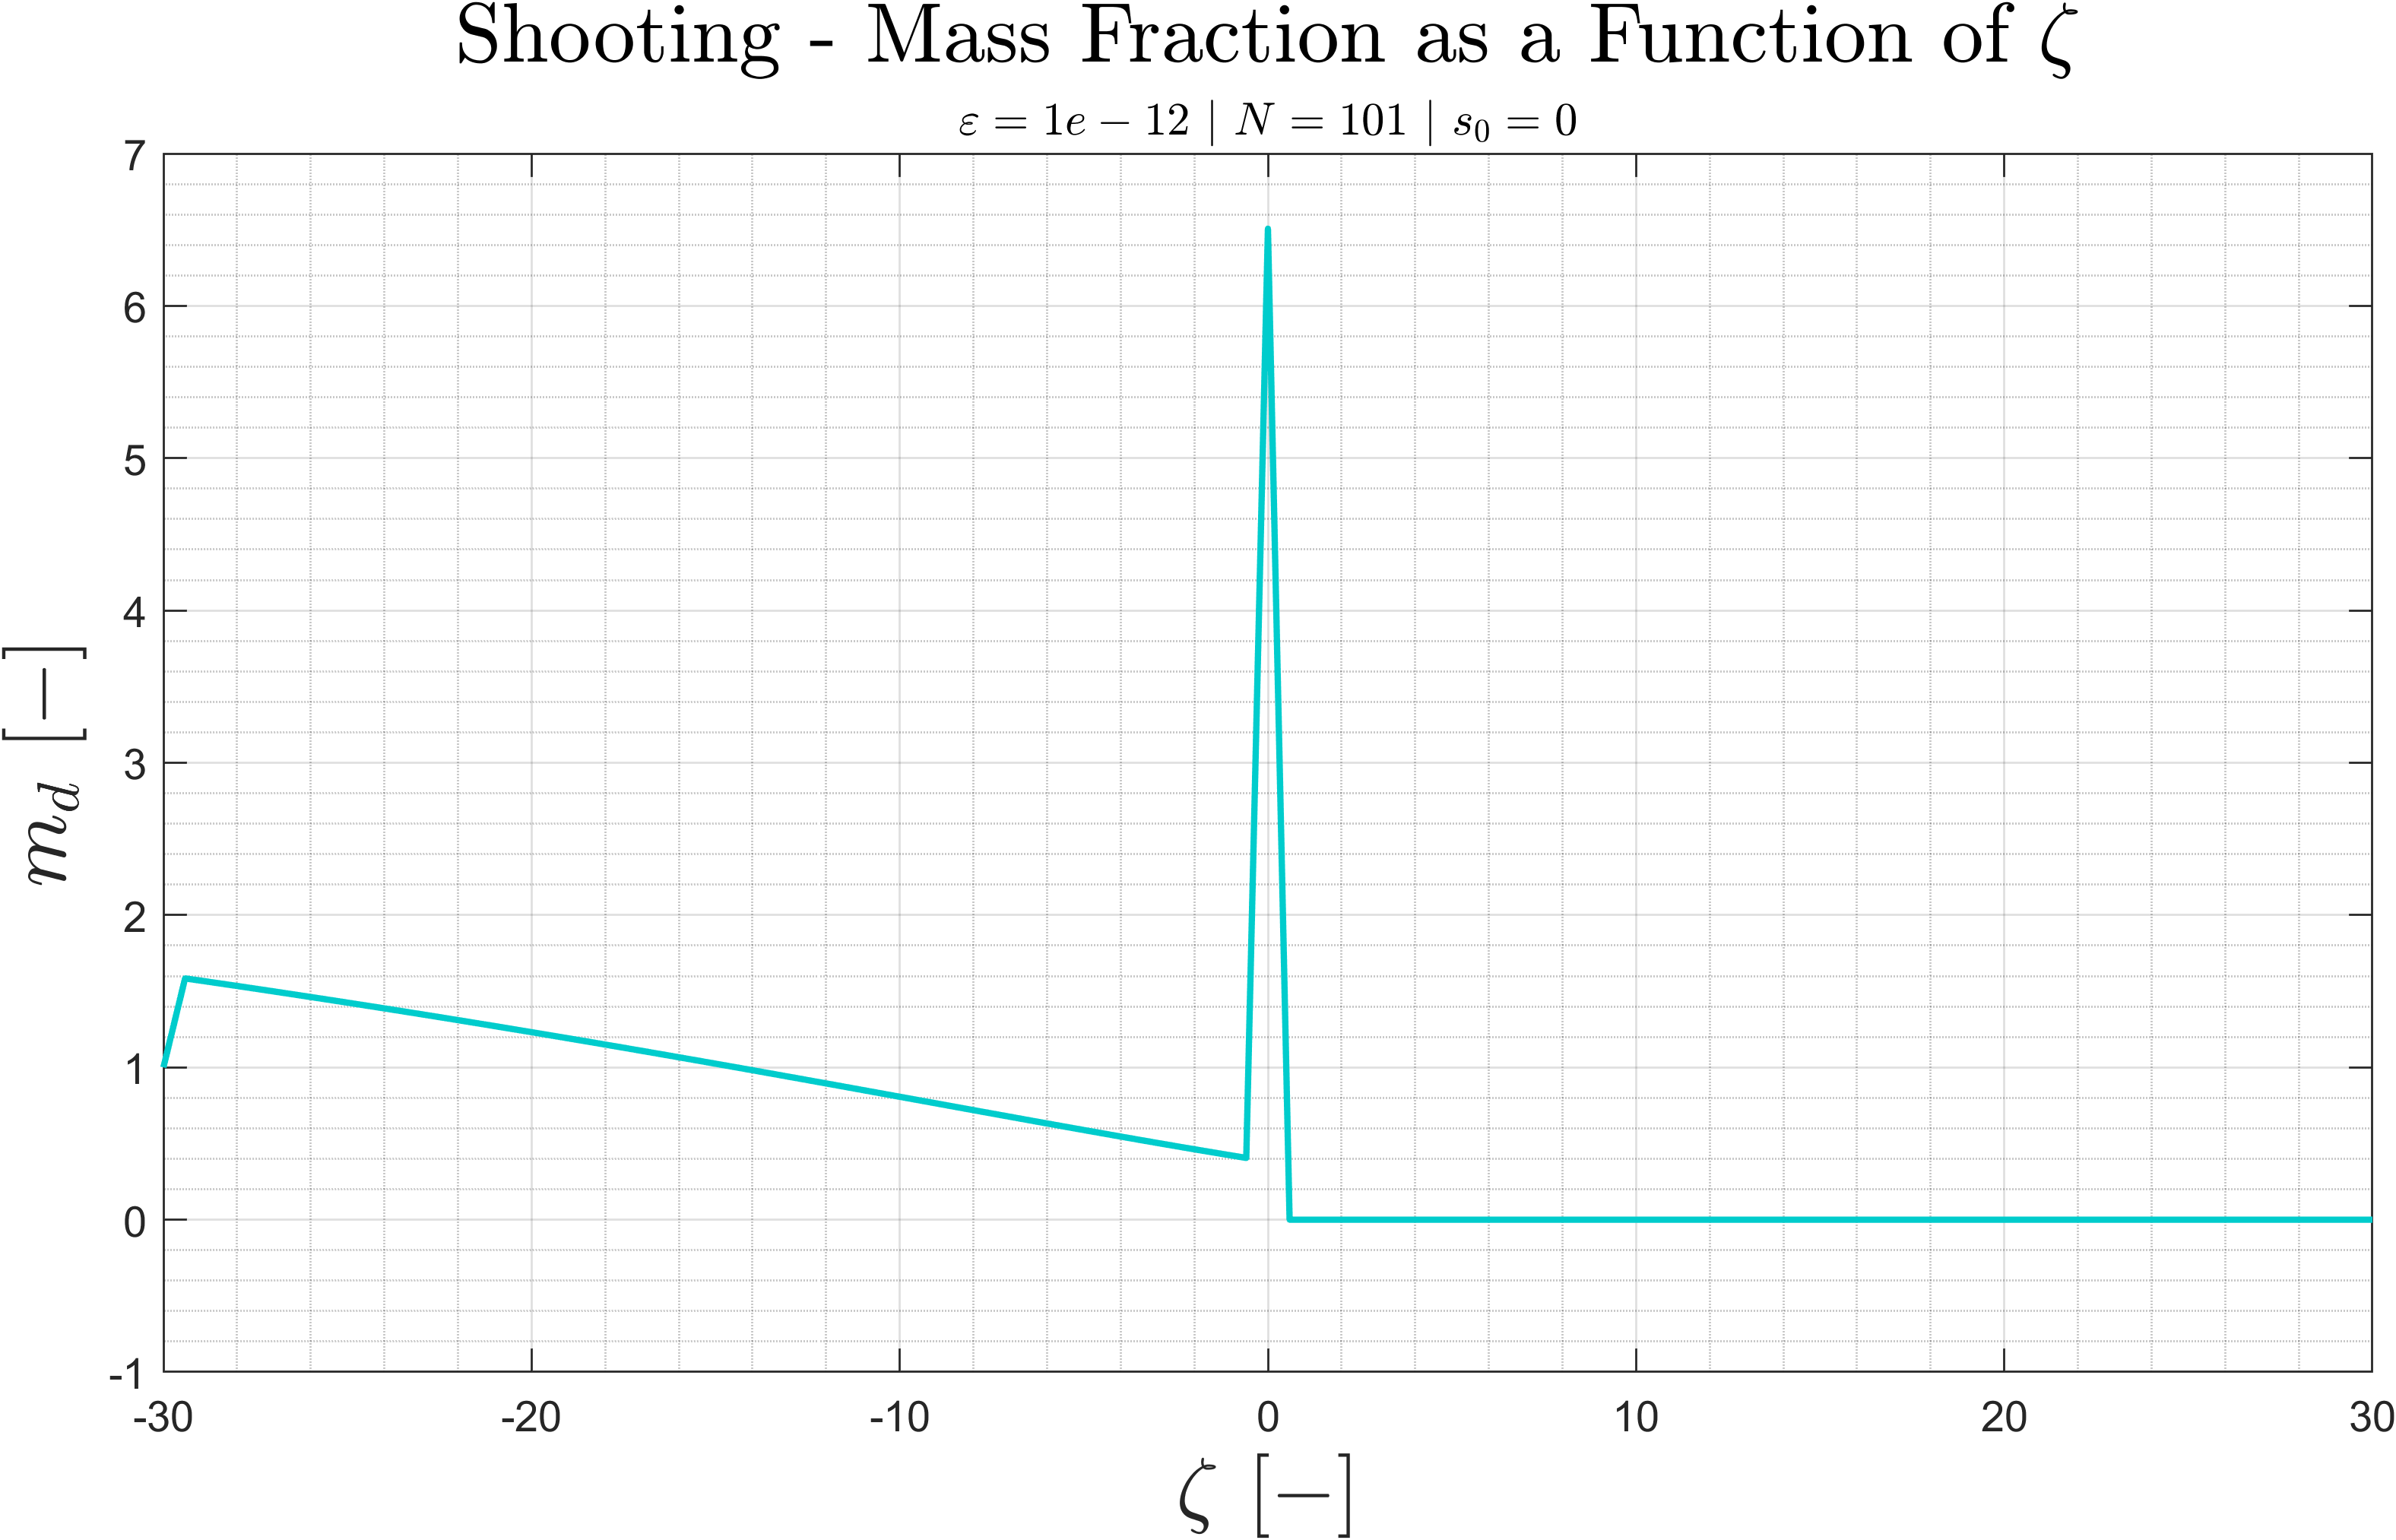
\includegraphics[width=\textwidth]{images/shooting - md vs zeta.png}
        \caption{shooting - mass fraction as a function of $\zeta$}
        \label{fig: shooting - md vs zeta}
    \end{subfigure}
    \begin{subfigure}[c]{0.55\textwidth}
        \centering
        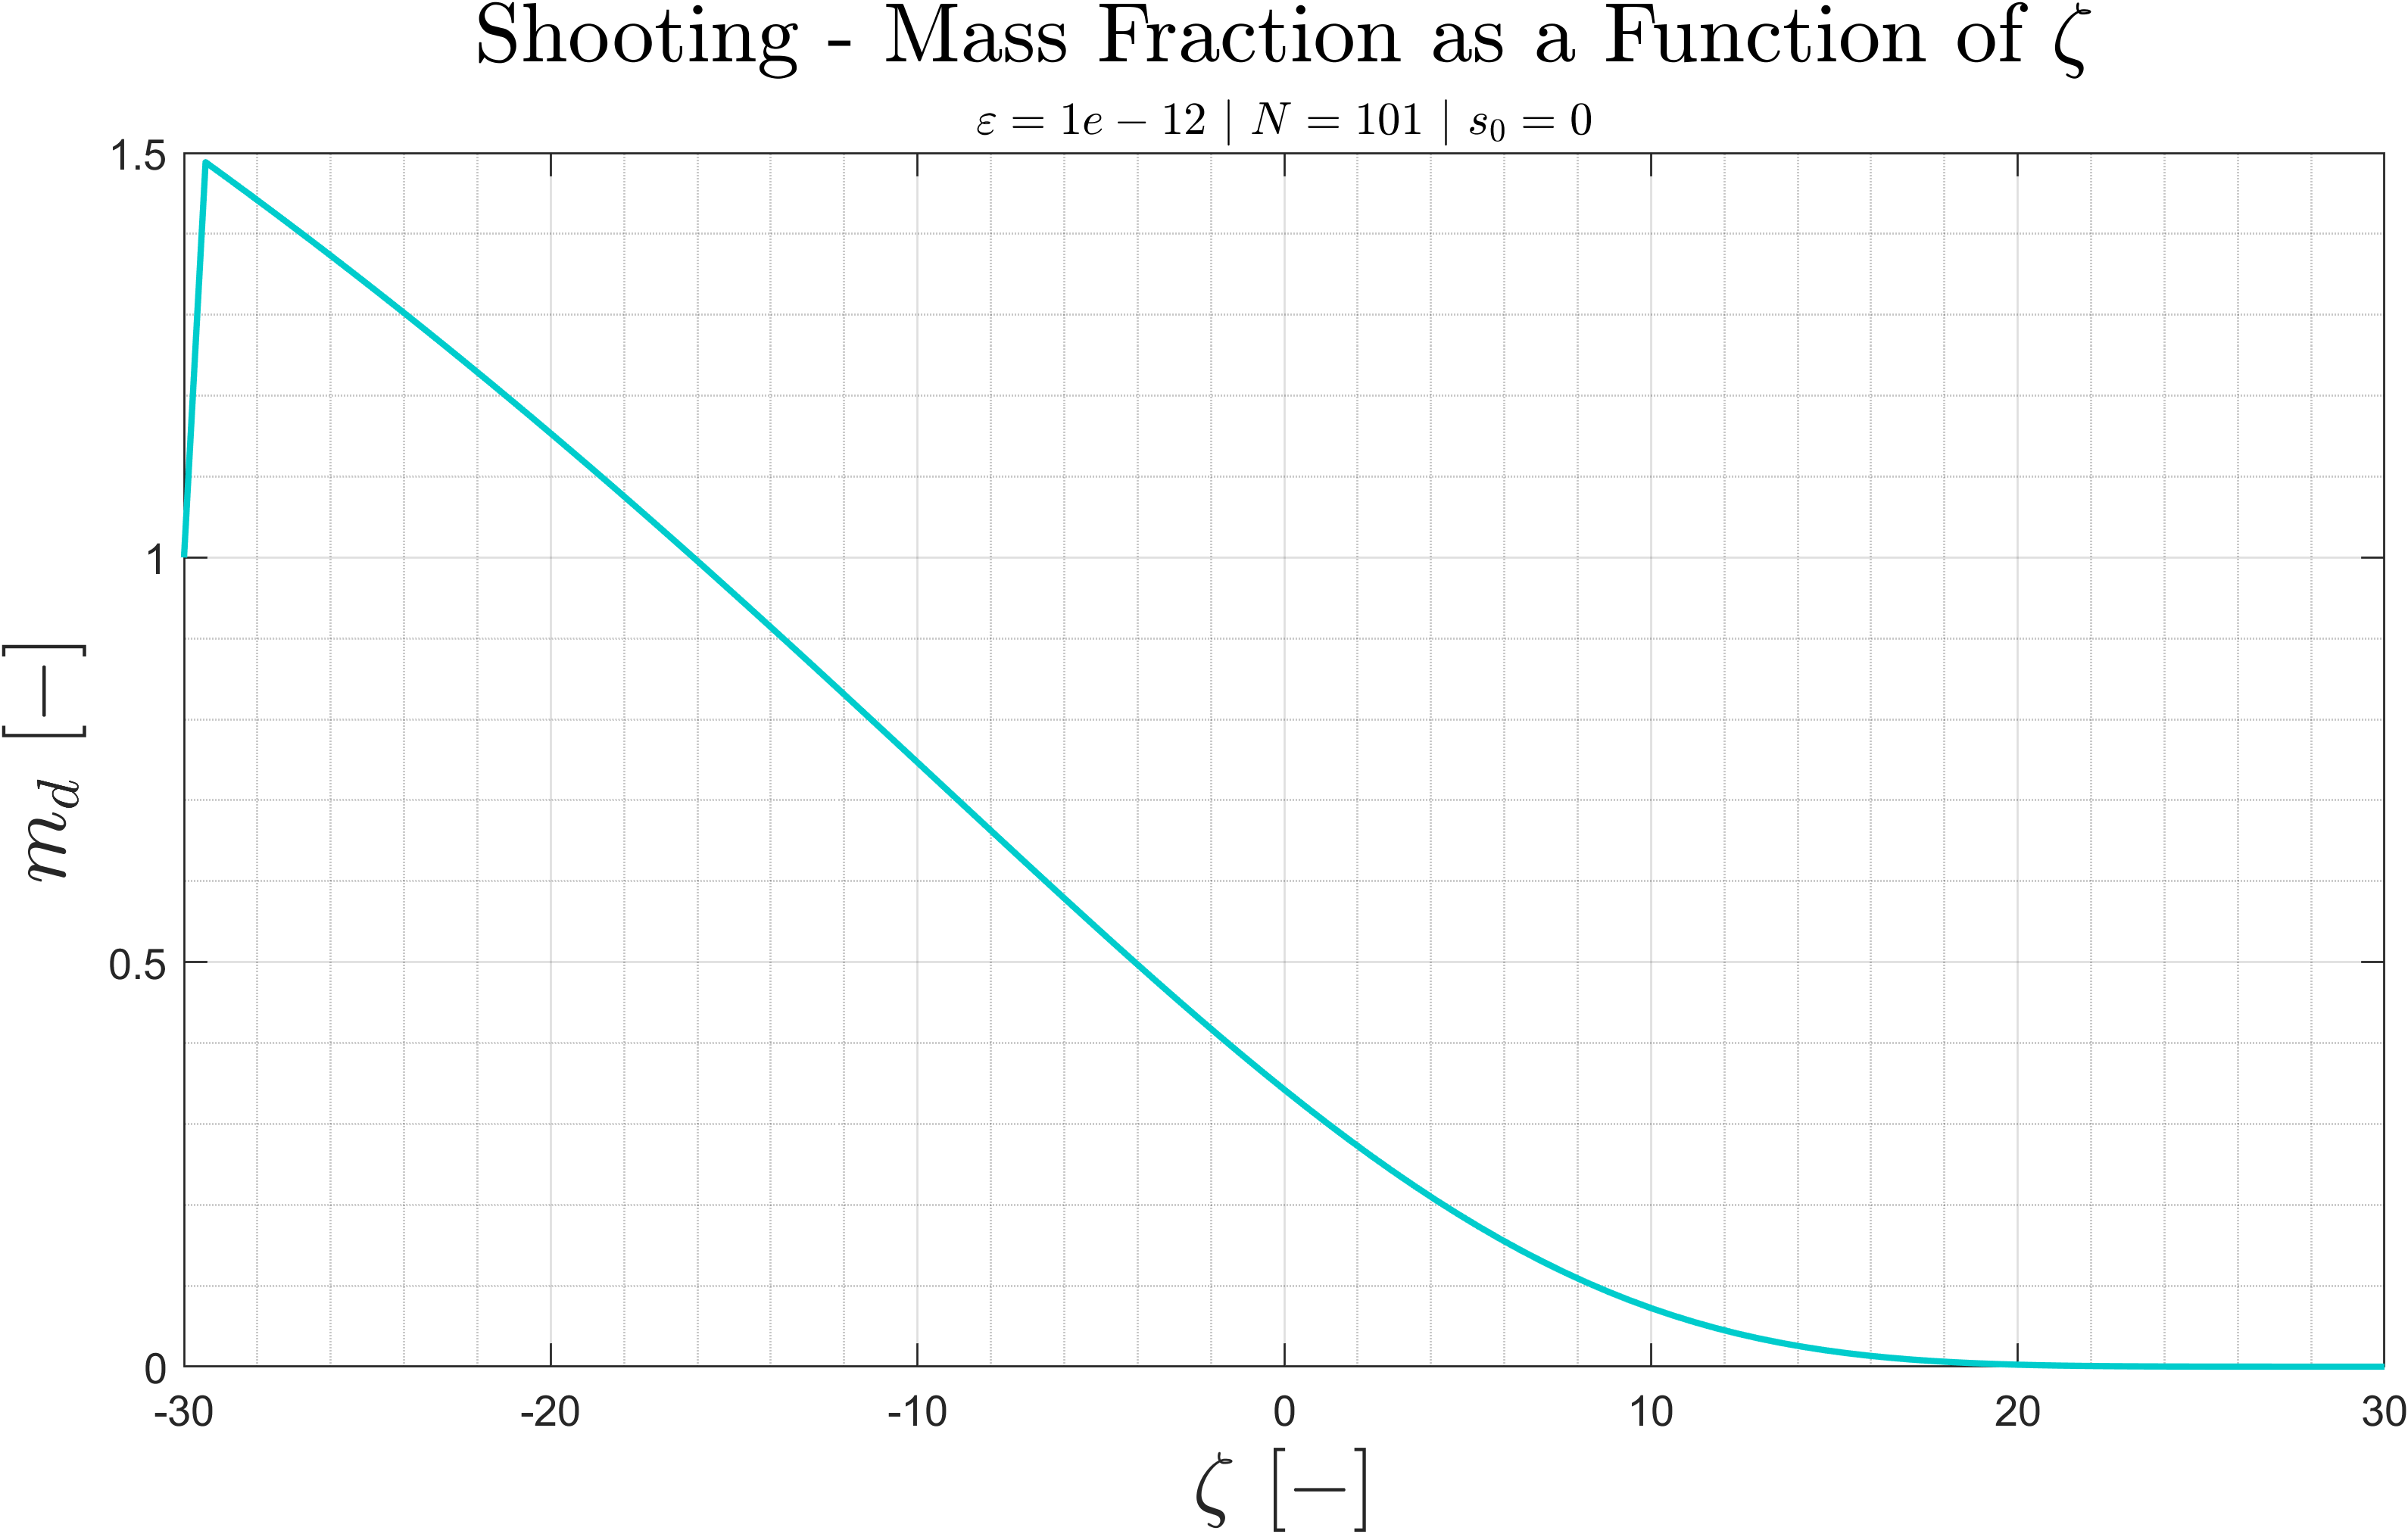
\includegraphics[width=\textwidth]{images/shooting - md vs zeta - no zero.png}
        \caption{shooting - mass fraction as a function of $\zeta$ - no zero}
        \label{fig: shooting - md vs zeta - no zero}
    \end{subfigure}
    \caption{Mass fraction as a function of $\zeta$}
    \label{fig: md vs zeta}
\end{figure}
\noindent In Fig.\ref{fig: md vs zeta} we can see that indeed for $\zeta>0$, the temperature is linear as the mass fraction is constant and depends on the second derivative of the temperature. Moreover, the forced $\left.T\right|_{\zeta=0}=0$ creates an artificial peak in the mass fraction, which causes it to have a single discontinuity. Additionally, the left boundary condition is not met as the analytically calculated boundary conditions for the temperature are only correct when $\zeta\rightarrow\pm\infty$.

\section{Summary and Conclusion}

\newpage
\appendix
\section{Listing of The Computer Program}
\subsection{Parameters}

\subsection{Main Code}

\end{document}